\chapter{Decapolar Fields}
\thumbforchapter{}
%\chaptertoc{}
%\newpage

% === Introduction
\section{Introduction}

% -----------------------
%       Motivation
\subsection{\review{Motivation}}

Beam-based measurements have been carried in the LHC since Run 1 to better understand the decapolar
fields. Those have been carried out via chromaticity
measurements~\cite{maclean_non-linear_2011,maclean_commissioning_2016,maclean_measurement_2014}. 
The third order of the non-linear chromaticity, $Q'''$, generated for the most part by decapoles,
has shown a consistent discrepancy at injection energy between its expected value from simulations
and that observed. Figure \ref{fig:decapoles:bare_chroma_vs_simulations} highlights this
discrepancy.

\begin{figure}[H]
    \centering
    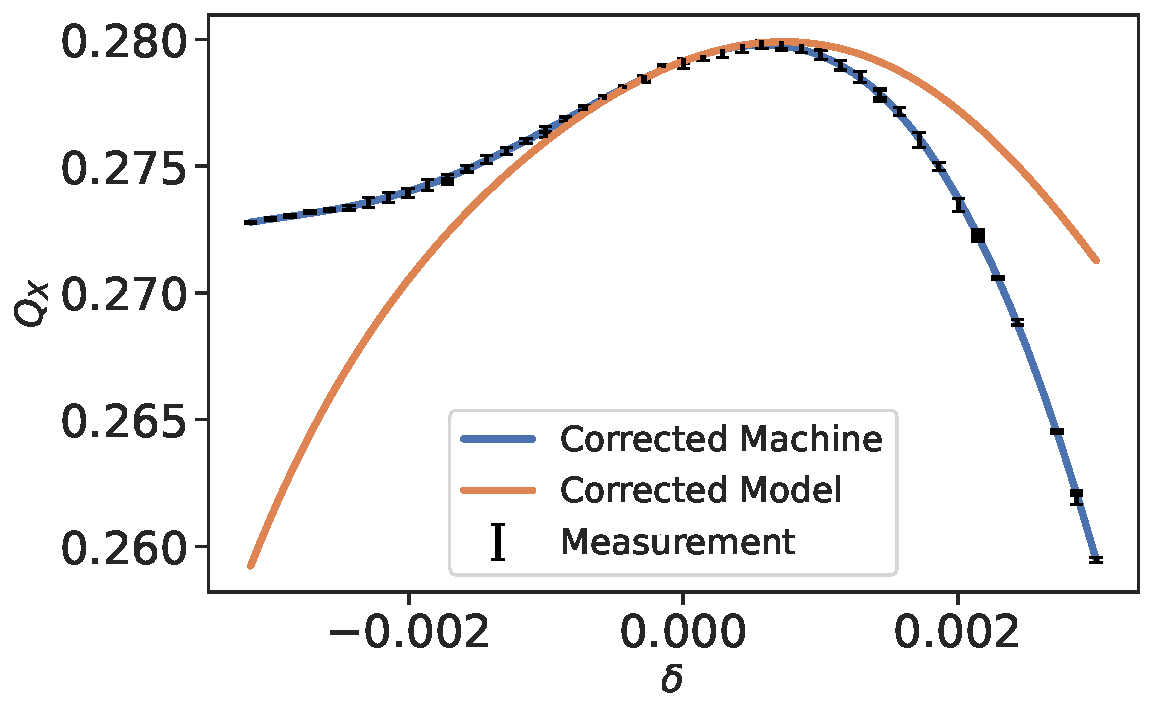
\includegraphics[width=0.8\textwidth]{images/dq3_corrected_simulation_fidel.pdf}
    \caption{Measured and simulated chromaticity with application of the nominal decapolar
    corrections from FiDeL. It can be seen that although the corrections should diminish $Q'''$, it
    is not well corrected in practice.}
    \label{fig:decapoles:bare_chroma_vs_simulations}
\end{figure}

The FiDeL magnetic model is used during operation to correct various multipole errors, including
octupolar and decapolar. The operational corrections being based on this magnetic model and
simulations, the residual $Q'''$ value is expected to be small, which is however not the case.
Chromaticity measurements have thus been repeated during LHC's Run 3 and corrections made routine,
aimed at correcting the observed discrepancy.

The study of non-linear chromaticity has proven valuable in quantifying decapolar fields, yet it
does not permit alone to understand the exact origins of the observed discrepancy. In an effort to
gain deeper insights, additional measurements were performed focusing on novel observables that had
not been previously explored.
\textit{Bare chromaticity} involves measuring chromaticity with
the octupolar an decapolar correctors deactivated ; this approach aims to isolate the machine
effects from those of the correctors.
\textit{Chromatic amplitude detuning}, evaluates how the tune varies with both the beam's action and
the momentum offset ; this methods has the benefit of having a different expression that of the
chromaticity.

Complementing those measurements, studies of decapolar Resonance Driving Terms have been undertaken
for the first time in the LHC. Contributing to resonances close to the working, those RDTs also have
benefited from corrections.


% --------------------------
%    Decapolar Correctors
\subsection{\review{Decapolar Correctors}}

As seen in \cref{fig:introduction:lhc_arc_cell}, the LHC is equipped with decapoles. Those magnets
are part of the design report, aiming at correcting the field errors of the main dipoles.
Those correctors, denominated \textit{MCD}, are specific to each beam and are placed after every
second dipole, totaling 1232 in number~\cite{venturini_delsolaro_magnetic_2005}.
MCDs are nested with octupolar correctors, \textit{MCO}. The pair of those correctors of often
referred to as \textit{MCDO}. 
It is not possible to individually power each corrector. Rather, a circuit consists of a whole arc.
There are in total 16 circuits to control the correctors of both beams and 8 arcs.
\cref{fig:decapoles:decapole_picture} shows a picture taken of decapoles on a test bench.

\begin{figure}
    \centering
    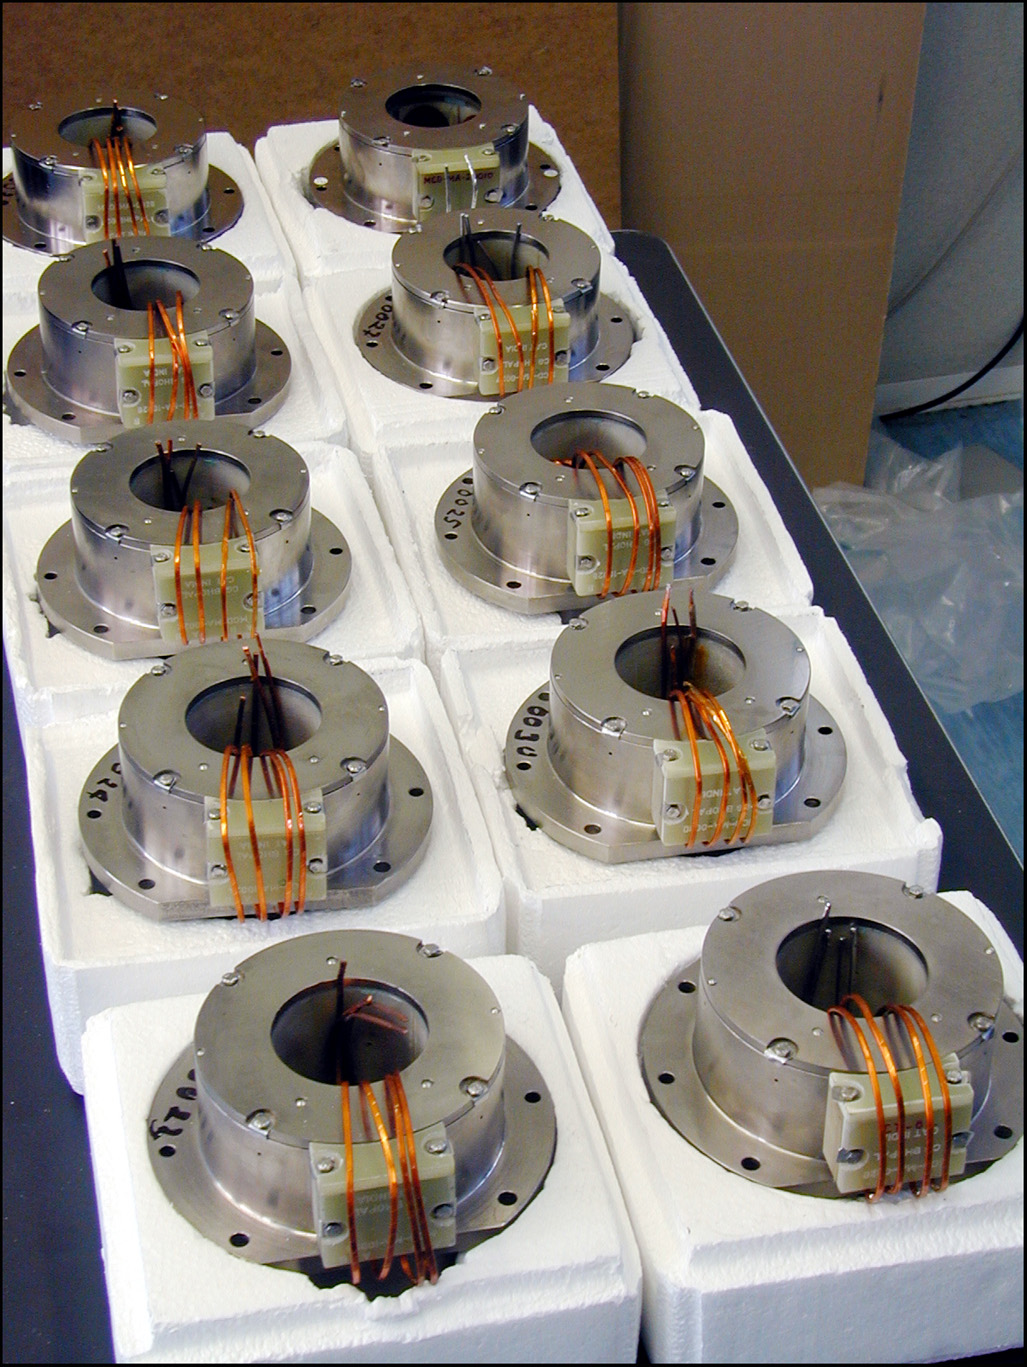
\includegraphics[width=0.4\textwidth]{./images/decapoles_real_pic.jpg}
    \caption{Decapoles on a test bench, being inspected after
    manufacturing~\cite{noauthor_ten_2001}.}
    \label{fig:decapoles:decapole_picture}
\end{figure}


The important characteristics of the magnetic fields of correctors are their main field transfer
function (or \textit{response}), the field quality and possible crosstalk, as MCOs and MCDs are
nested~\cite{venturini_delsolaro_magnetic_2005}.
In order to better understand the decapolar fields, the decapole correctors themselves need to be
studied.


% -------- Strengths at Injection
\paragraph{Strengths at Injection}

%\begin{wraptable}{r}{0.4\textwidth}
\begin{table}
    \centering
    \begin{tabular}{lr}
        \toprule
        Circuit   & $K_5 [\textrm{m}^{-5}]$ \\
        \midrule
        Beam 1    & \\
        \hspace{2mm}RCD.A12B1 & $-4582$ \\
        \hspace{2mm}RCD.A23B1 & $-5106$ \\
        \hspace{2mm}RCD.A34B1 & $-4855$ \\
        \hspace{2mm}RCD.A45B1 & $-4577$ \\
        \hspace{2mm}RCD.A56B1 & $-4125$ \\
        \hspace{2mm}RCD.A67B1 & $-5166$ \\
        \hspace{2mm}RCD.A78B1 & $-6827$ \\
        \hspace{2mm}RCD.A81B1 & $-5500$ \\
        Beam 2    & \\
        \hspace{2mm}RCD.A12B2 & $-4490$ \\
        \hspace{2mm}RCD.A23B2 & $-5155$ \\
        \hspace{2mm}RCD.A34B2 & $-4825$ \\
        \hspace{2mm}RCD.A45B2 & $-4619$ \\
        \hspace{2mm}RCD.A56B2 & $-4064$ \\
        \hspace{2mm}RCD.A67B2 & $-5066$ \\
        \hspace{2mm}RCD.A78B2 & $-6866$ \\
        \hspace{2mm}RCD.A81B2 & $-5446$ \\
        \bottomrule
    \end{tabular}
    \caption{Strength of decapolar correctors at injection energy for FiDeL corrections.}
    \label{tab:decapoles:strength_rcd_fidel}
%\end{wraptable}
\end{table}

At injection energy, the decapoles are powered to a static strength. New optics introduced
throughout the years often have for effect to vary slightly the $\beta$-function along the ring,
having thus an impact on the chromaticity, as seen in
\cref{eq:detuning_effects:chromaticity_strength}. New corrections are then computed via FiDeL to
account for it.
Although those corrections vary throughout the years, the shift is in practice fairly negligible.
\cref{tab:decapoles:rdts:correction_f1004_k5}, a bit further in this chapter, shows the strength of
the correctors and the related circuits at injection energy for the optics deployed in 2024.


% ===================
%    Chromaticity
% ===================


% Correction
%\paragraph{Correction}
%
%$Q'''$ is linear with the decapole strength. As such, it can be easily corrected via global trims
%presented in~\cref{subsection:correction_chromaticity}.
%A change of decapole strength $K_5 = 1000$ would for example have the following impact with the
%injection optics used in 2022:
%
%\begin{equation}
%    \begin{aligned}
%        \Delta Q'''_x =  1.5 \times 10^6 \quad;\quad
%        \Delta Q'''_y = -0.9 \times 10^6.
%    \end{aligned}
%\end{equation}






%\subsection{\todo{blabla}}
%
%Measurements were taken during 2022 Commissioning for 
%\begin{itemize}
%    \item Beam Test
%    \item Commissioning
%    \begin{itemize}
%        \item FiDeL
%        \item Q''' corr
%        \item Q'' corr
%    \end{itemize}
%    \item 60° optics
%\end{itemize}
%
%Also during MD6864, 2022-10-19, for the bare machine \\
%Also 2022-11-06, measurement at 30cm, flat top.
%

% ===============================
%        Corrector Response
% ===============================
\section{\review{Response of correctors}}

% ===============================
%         Introduction
\paragraph{Expression}

The full third term of the chromaticity function is highlighted in
\cref{eq:decapoles:chromaticity_highlight}. Details on chromaticity are given
in \cref{subsection:concepts:chromaticity}.

\begin{equation} 
    Q (\delta) = Q_0 + Q' \delta + \frac{1}{2!} Q'' \delta^2 
                     + \colorbox{yellow!50}{$\displaystyle  \frac{1}{3!}  Q''' \delta^3$}
                     + \mathcal{O}(\delta^4).
    \label{eq:decapoles:chromaticity_highlight}
\end{equation}

This third order, mainly contributed to by decapoles, is related to the $\beta$-function, the
dispersion and the strength of the multipole:

\begin{equation}
    \begin{aligned}
        \Delta Q_x''' &=  &\frac{1}{4\pi} K_{5} L \beta_x D_x^{3}\\
        \Delta Q_y''' &= -&\frac{1}{4\pi} K_{5} L \beta_x D_x^{3}.
    \end{aligned}
\end{equation}


% 2022-04-24
\paragraph{Measurements and Corrections}

In order to assess the accuracy of corrections, measurements have to be done to gauge the response
of the decapolar correctors, \textit{MCDs}.
During Run~3's commissioning, measurements and corrections of $Q''$ and $Q'''$ have been made
routine. Those corrections give the opportunity to study the response of the correctors.
\cref{figure:decapoles:chromaticity:dq3_comparison} shows the chromaticity function measured during
Run~3's commissioning in 2022 with the nominal corrections via FiDeL and beam-based corrections
computed analytically based on top of FiDeL.

\begin{figure}[H]
    \centering
    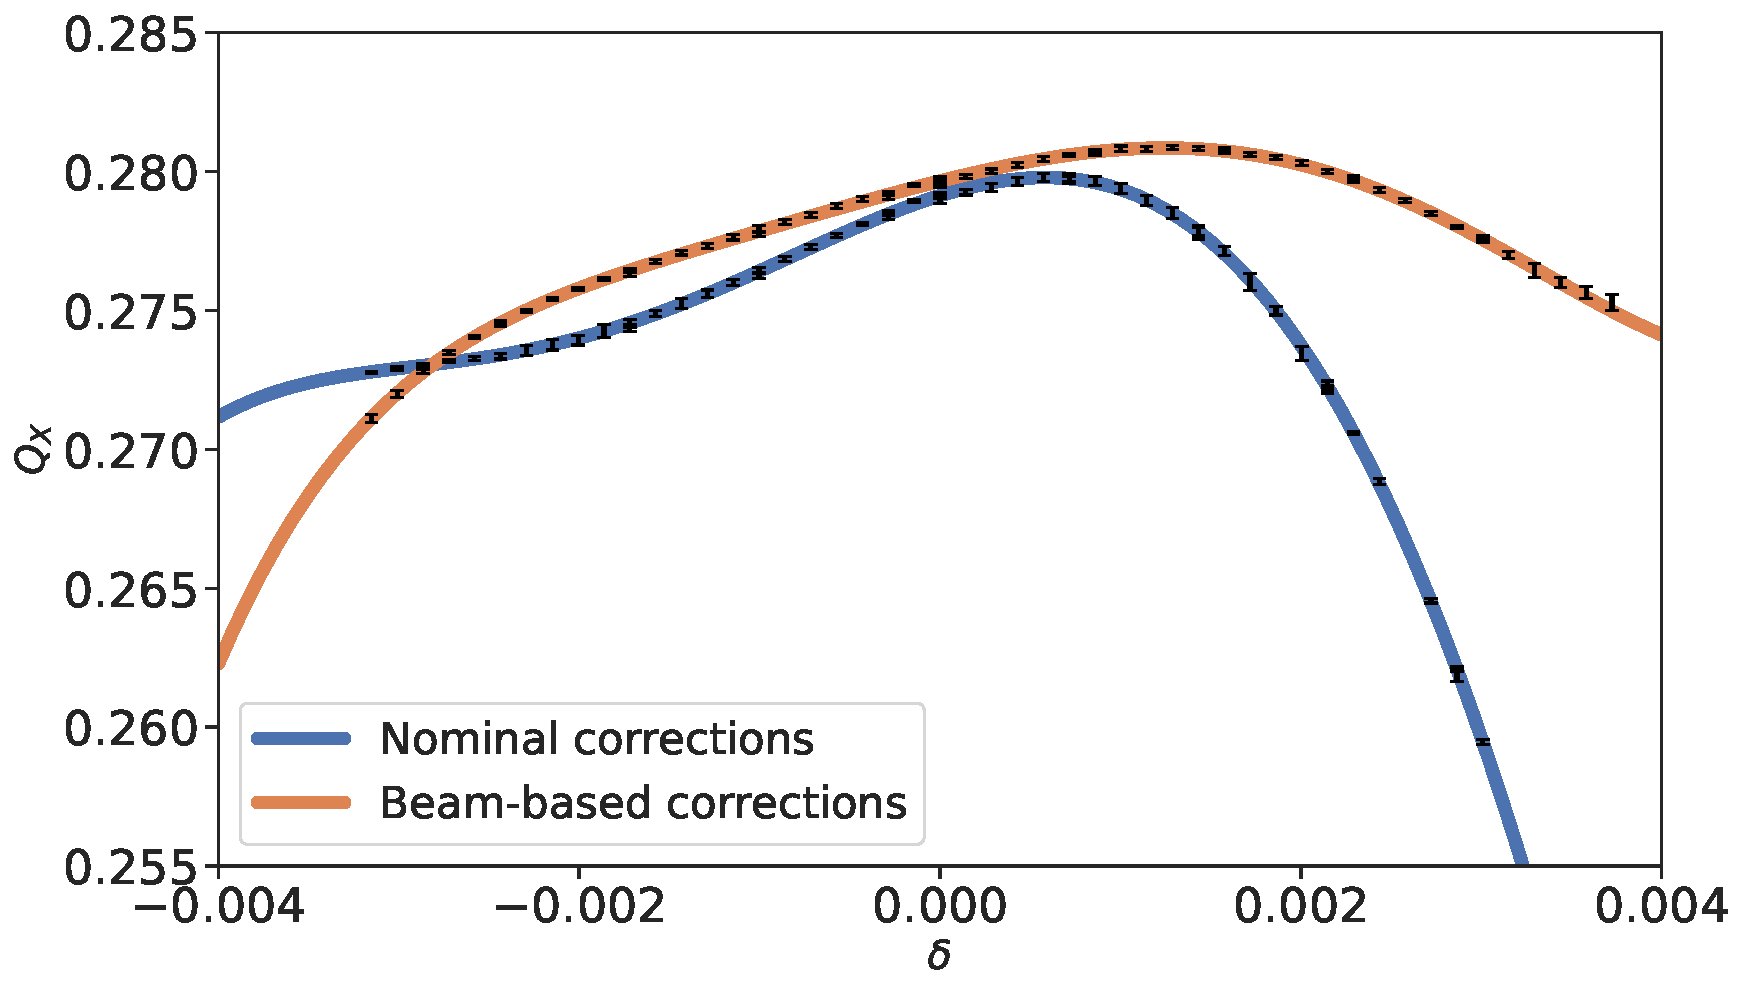
\includegraphics[width=0.8\columnwidth]{images/nominal_vs_beam_based_corrections.pdf}
    \caption{Chromaticity of the horizontal plane of Beam 1 during Run 3's commissioning, with
    nominal corrections based on the magnetic model and beam-based corrections aimed at correcting
     $Q''$ and $Q'''$.}
    \label{figure:decapoles:chromaticity:dq3_comparison}
\end{figure}

The nominal and corrected $Q'''$ values are shown in
\cref{table:decapoles:chromaticity:dq3_before_after_beam_based}. The shift in $Q'''$ is shown for
each beam and axis, showing a good agreement between the measurement and the simulation.
The slight imbalance can be attributed to higher order effects of the octupole correctors, whose
correction was implemented after that of $Q'''$.

\begin{table}[H]
    \centering
    \begin{tabular}{|l||r|r|r|c|}
    \hline
              &  \multicolumn{2}{c|}{$Q''' [10^6]$}  &  \multicolumn{2}{c|}{$\Delta Q''' [10^6]$}\\ \hline\hline
        B1    &   \multicolumn{1}{c|}{Nominal}     &   \multicolumn{1}{c|}{Beam-based}   & Measured & Simulated \\
        X     &  -3.36 ± 0.04 &  -1.02 ± 0.03  &  2.3 ± 0.1 &   2.5 \\
        Y     &   1.62 ± 0.05 &   0.12 ± 0.02  & -1.5 ± 0.1 &  -1.4 \\ \hline
        %B2    &   \multicolumn{1}{c|}{Nominal}     &   \multicolumn{1}{c|}{Beam-based}   &&\\
        B2    &               &&& \\
        X     &  -2.72 ± 0.08 &  -0.64 ± 0.03  &  2.1 ± 0.1 &  2.5\\
        Y     &   1.54 ± 0.06 &   0.14 ± 0.03  & -1.4 ± 0.1 & -1.4\\ \hline
    \end{tabular}
    \caption{Third order chromaticity obtained during Run~3 commissioning, with nominal and
    beam-based corrections aimed at correcting $Q''$ and $Q'''$.
    The change in $Q'''$, measured and expected via simulations, is also shown.} 
    \label{table:decapoles:chromaticity:dq3_before_after_beam_based}
\end{table}


This agreement between the simulations and the measurements indicates that our decapole correctors
function as intended. No noticeable cross-talk between magnets or hysteresis have been identified.



% ===============================
%        Bare Chromaticity
% ===============================
\section{\review{Bare Chromaticity}}


% 2022-10-19

Previous studies~\cite{maclean_measurement_2014} have demonstrated that octupole and decapole
correctors were contributing to an observed octupolar discrepancy in the machine via hysteresis and
feed-down. To evaluate the possible effect of decapole correctors on the third order chromaticity
$Q'''$, a measurement was taken with these elements turned off.

\begin{figure}[H]
    \begin{subfigure}{0.49\textwidth}
        \centering
        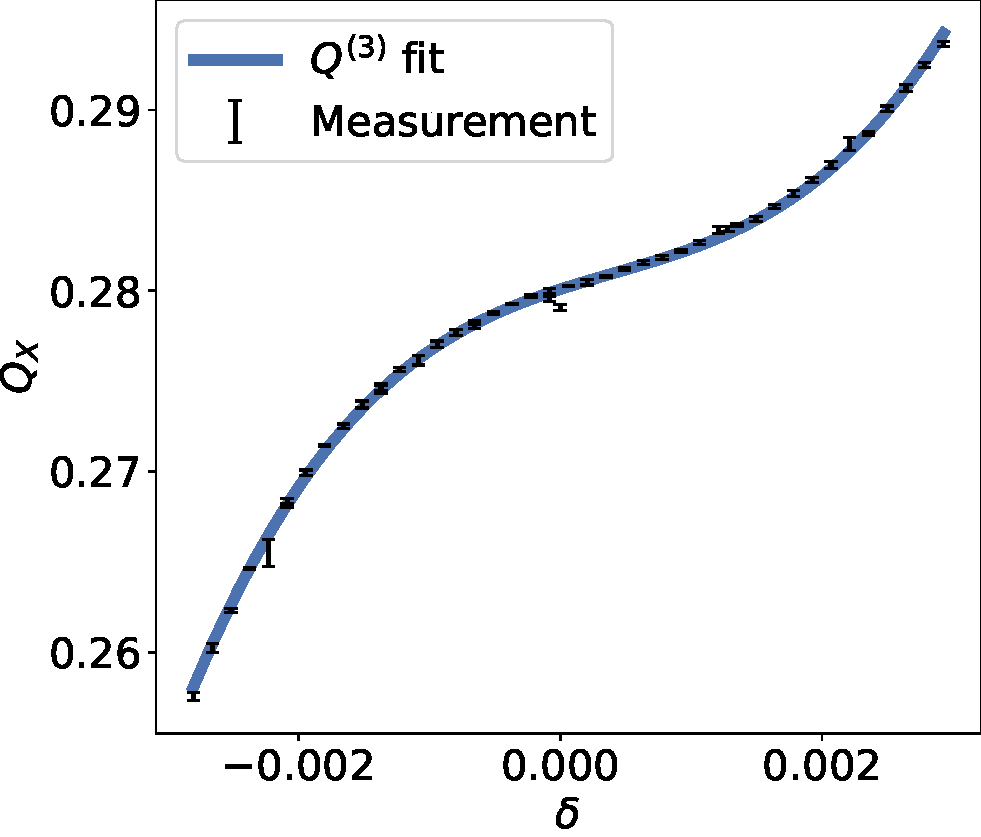
\includegraphics[width=\textwidth]{./images/bare_chromaticity/Beam1_Qx.pdf}
        \caption{$Q_x$ Beam 1}
        \label{}
    \end{subfigure}
    \hfill
    \begin{subfigure}{0.49\textwidth}
        \centering
        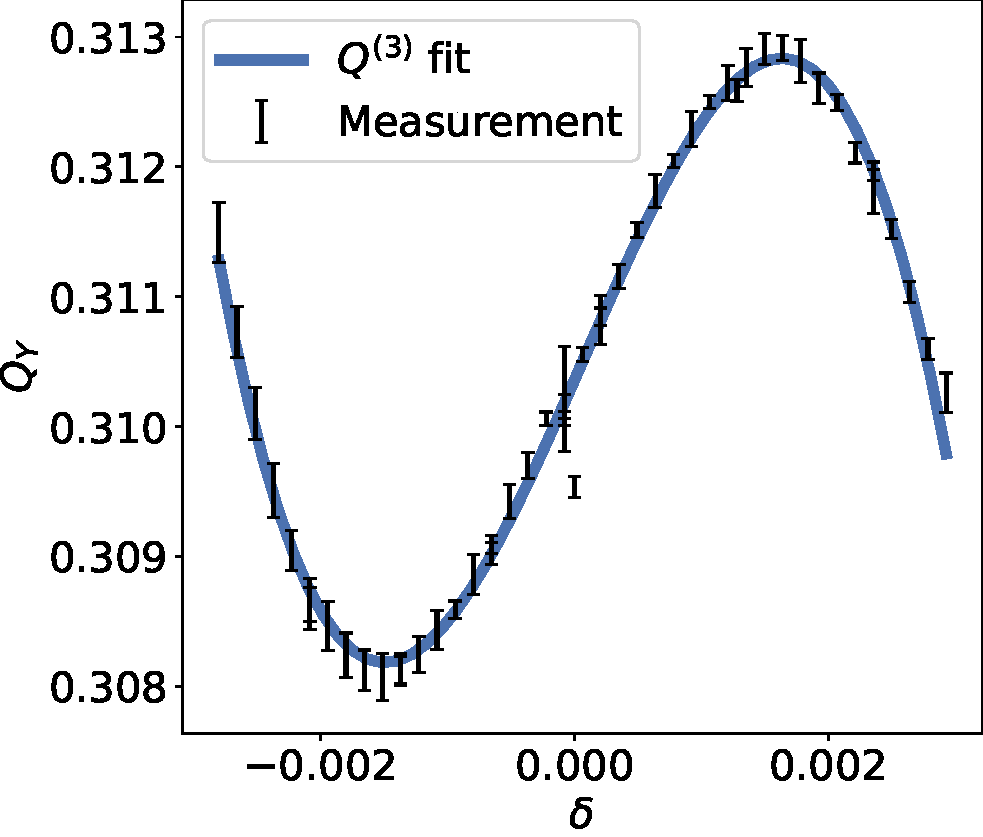
\includegraphics[width=\textwidth]{./images/bare_chromaticity/Beam1_Qy.pdf}
        \caption{$Q_y$ Beam 1}
        \label{}
    \end{subfigure}
    %
    \\
    %
    \begin{subfigure}{0.49\textwidth}
        \centering
        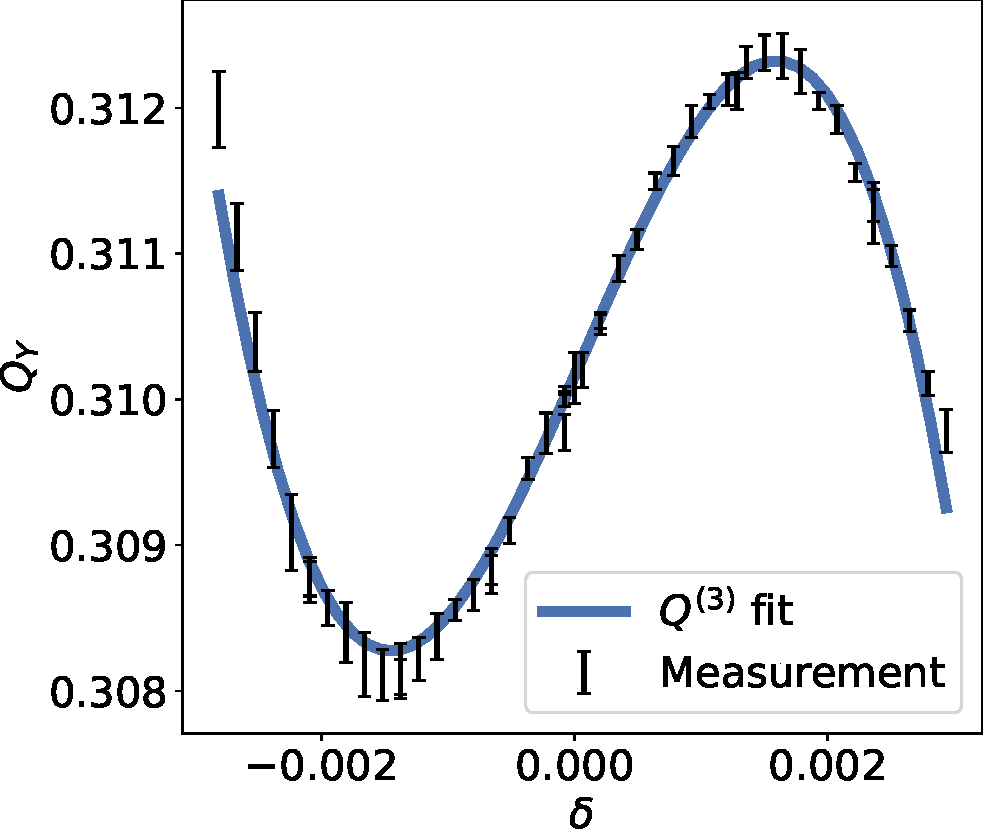
\includegraphics[width=\textwidth]{./images/bare_chromaticity/Beam2_Qy.pdf}
        \caption{$Q_x$ Beam 2}
        \label{}
    \end{subfigure}
    \hfill
    \begin{subfigure}{0.49\textwidth}
        \centering
        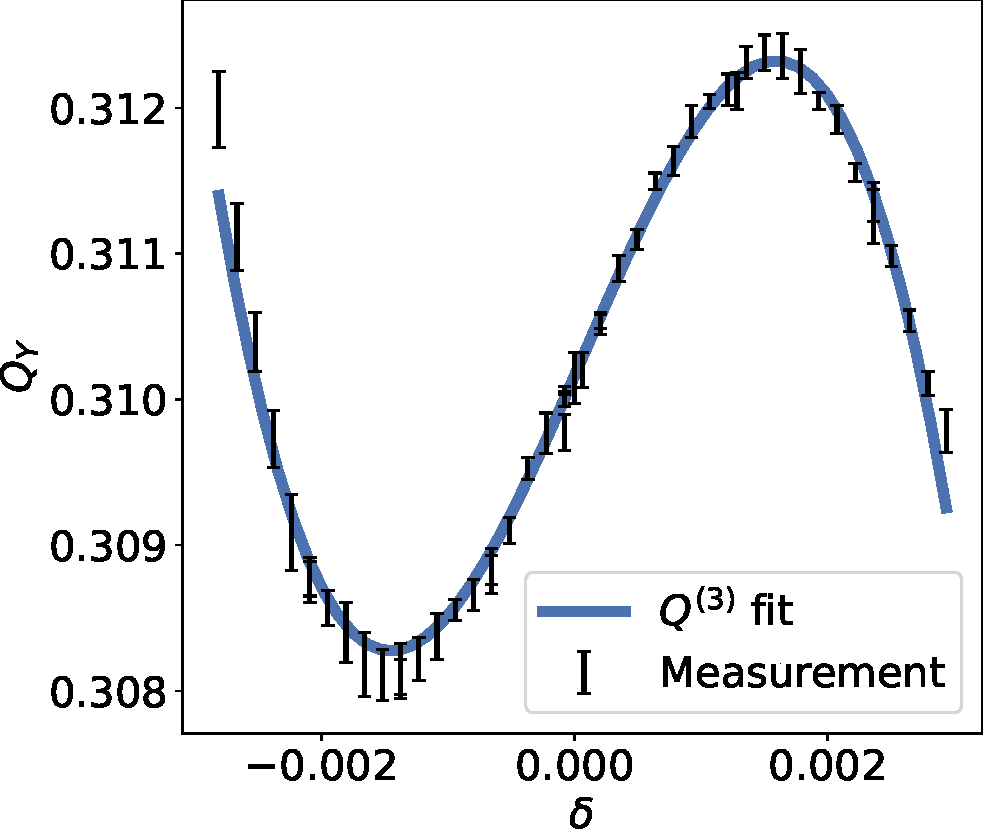
\includegraphics[width=\textwidth]{./images/bare_chromaticity/Beam2_Qy.pdf}
        \caption{$Q_y$ Beam 2}
        \label{}
    \end{subfigure}
    \caption{Fit of the chromaticity function for the chromaticity measurement performed with 
    octupole and decapole correctors powered off. The fit includes all orders up to third.}
    \label{fig:decapoles:bare_chromaticity}
\end{figure}

Simulations have been run with MAD-X and PTC including fields errors from $b_3$ to $b_8$. The
expected $Q'''$ values are presented in~\cref{table:decapoles:bare_chromaticity:virgin_dq3} and
compared to the measured ones along with the ratio between the two.

\begin{table}[tbh]
    \centering
    \begin{tabular}{|l||r|r|r|}
    \hline
        Plane     &  Meas. $Q''' [10^6]$        &  Sim. $Q''' [10^{6}]$          &   Ratio     \\\hline\hline
        Beam 1    &                             &                                &             \\
                X &            2.95 ± 0.04      &         6.94 ± 0.02            &  0.43 ± 0.01  \\
                Y &           -1.82 ± 0.04      &        -4.29 ± 0.01            &  0.42 ± 0.01  \\ \hline
        Beam 2    &                             &                                &             \\
                X &            3.06 ± 0.07      &        7.03 ± 0.02             &  0.44 ± 0.01 \\
                Y &           -1.72 ± 0.02      &       -4.27 ± 0.01             &  0.42 ± 0.01  \\ \hline
    \end{tabular}
    \caption{Measured and simulated third order chromaticity with octupole and decapole correctors
    turned off. The simulations include field errors from sextupoles to decahexapole ($b_3$ to
    $b_8$).}
    \label{table:decapoles:bare_chromaticity:virgin_dq3}
\end{table}

A consistent ratio is observed for every plane and axis between the measurement and the model. This
result, supplemented by the correct response of the correctors, indicates that the decapolar
correctors do no generate unwanted fields. Those correctors can thus be discarded as the potential
source of discrepancy.


%==================================
%   Chromatic Amplitude Detuning
%==================================
% ###################################
%      Chromatic Amplitude Detuning
\section{\review{Chromatic Amplitude Detuning}}

The Chromatic Amplitude Detuning is the tune shift dependant on both the actions and the momentum
offset, whose decapole contributed terms are described via a Taylor expansion in
\cref{eq:decapoles:chromatic_ampdet:decapole_contribution}. More information and derivations can
be found in \cref{subsection:detuning_effects:chromatic_amplitude_detuning} and
\cref{appendix:chromatic_amplitude_detuning}.

\begin{equation}
  \begin{aligned}
    \Delta Q(J_x, J_y, \delta) = 
    & \frac{\partial^2Q}{\partial J_x \partial \delta}    \cdot J_x\delta 
    + \frac{\partial^2 Q}{\partial J_y \partial \delta}   \cdot J_y\delta 
    + \frac{1}{3!} \frac{\partial^3 Q}{\partial \delta^3} \cdot \delta^3.
    \end{aligned}
    \label{eq:decapoles:chromatic_ampdet:decapole_contribution}
\end{equation}


The last term is more commonly referred to as the third order chromaticity, $Q'''$.  Each of those
terms depend on the $\beta$-functions, the horizontal dispersion $D$ and the normalized decapole
field gradient $K_5$ for a single source of length $L$,

\begin{equation}\begin{aligned}
  \frac{\partial^2 Q_x}{\partial J_x \partial \delta} =& \frac{1}{16 \pi} K_5L \beta_x^2 D,         &\quad
  \frac{\partial^2 Q_x}{\partial J_y \partial \delta} =& -\frac{1}{8\pi} K_5L \beta_x \beta_y D,
\\
  \frac{\partial^3 Q_x}{\partial \delta^3}            =& \frac{1}{4\pi} K_5L \beta_x D^3,           &\quad
  \frac{\partial^2 Q_y}{\partial J_x \partial \delta} =& -\frac{1}{8\pi} K_5L \beta_x \beta_y D,
\\
  \frac{\partial^2 Q_y}{\partial J_y \partial \delta} =& \frac{1}{16 \pi} K_5L \beta_y^2 D,        &\quad 
  \frac{\partial^3 Q_y}{\partial \delta^3}            =& -\frac{1}{4\pi} K_5L \beta_y D^3.
\end{aligned}\end{equation}

The action dependant terms can be measured by exciting the beam with an AC-dipole with increasing
strengths at different momentum-offsets.

Such a measurement was taken with octupole and decapole correctors turned off to measure the bare
machine. Some data could not be collected due to machine availability issues, restricting the
measurement to low intensity kicks. 
Nevertheless, the terms $\frac{\partial^2 Q_x}{\partial J_y \partial \delta}$ and $\frac{\partial^2
Q_y}{\partial J_y \partial \delta}$ for beam 2 were measured for the first time in the LHC. The
momentum-offsets measured at were $-0.001$ and $0.001$, respectively roughly equal to a trim of 
$+140$Hz and $-140$Hz of the RF.

\cref{figure:decapoles:chromatic_amplitude_detuning:b2qxy}
and~\cref{figure:decapoles:chromatic_amplitude_detuning:b2qyy} show a fit of those terms to measured
$Q_{x,y}$ vs $J_{y}$ at two different momentum offsets. Expected shifts from MADX-PTC simulations,
that include field errors ranging from sextupoles to decahexapoles ($b_3$ to $b_8$ and $a_4$ to
$a_8$) are shown as a comparison.

% Studies and plots in 
% jupyter/chromatic_amplitude_detuning/simulations/2022-10-19_vs_PTC/Analytical_Chromatic_Detuning.ipynb

\begin{figure}[H]
  \centering
  \begin{subfigure}{0.8\textwidth}
      \centering
      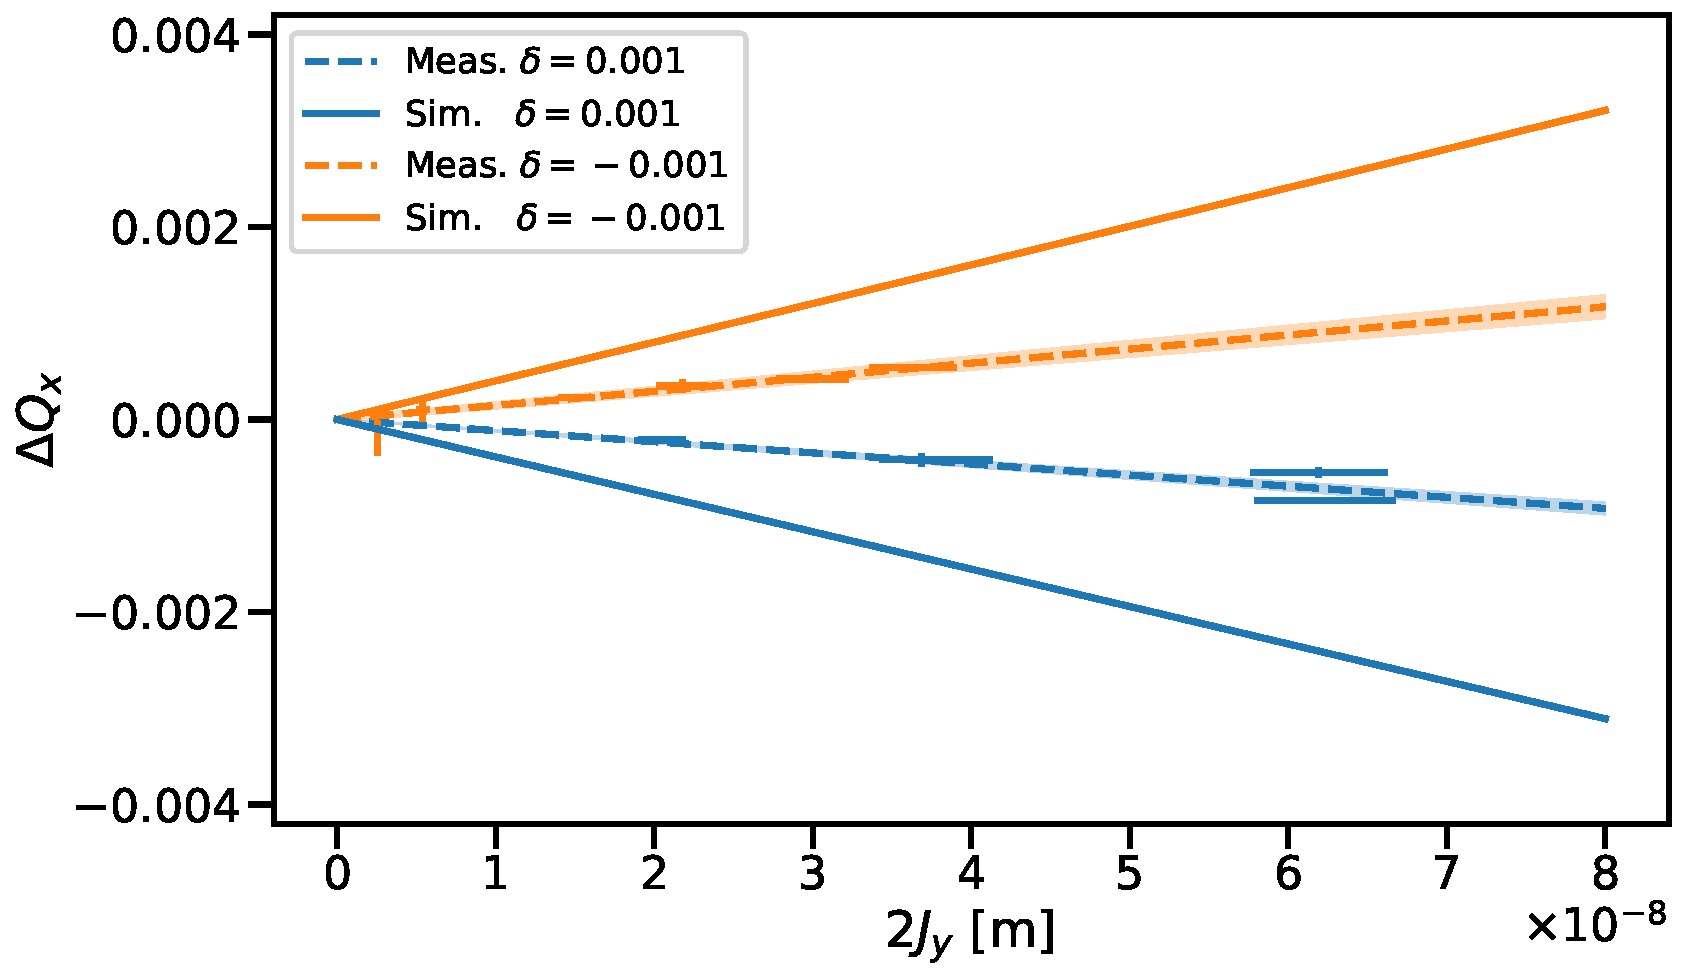
\includegraphics[width=\textwidth]{images/chromatic_amplitude_detuning/B2_Qxy_decay0.00.pdf}
      \caption{Horizontal tune shift depending on the vertical action: 
      $\frac{\partial^2 Q_x}{\partial J_y \partial \delta}$.}
      \label{figure:decapoles:chromatic_amplitude_detuning:b2qxy}
  \end{subfigure}
  %
  \\[1em]
  %
  \begin{subfigure}{0.8\textwidth}
      \centering
      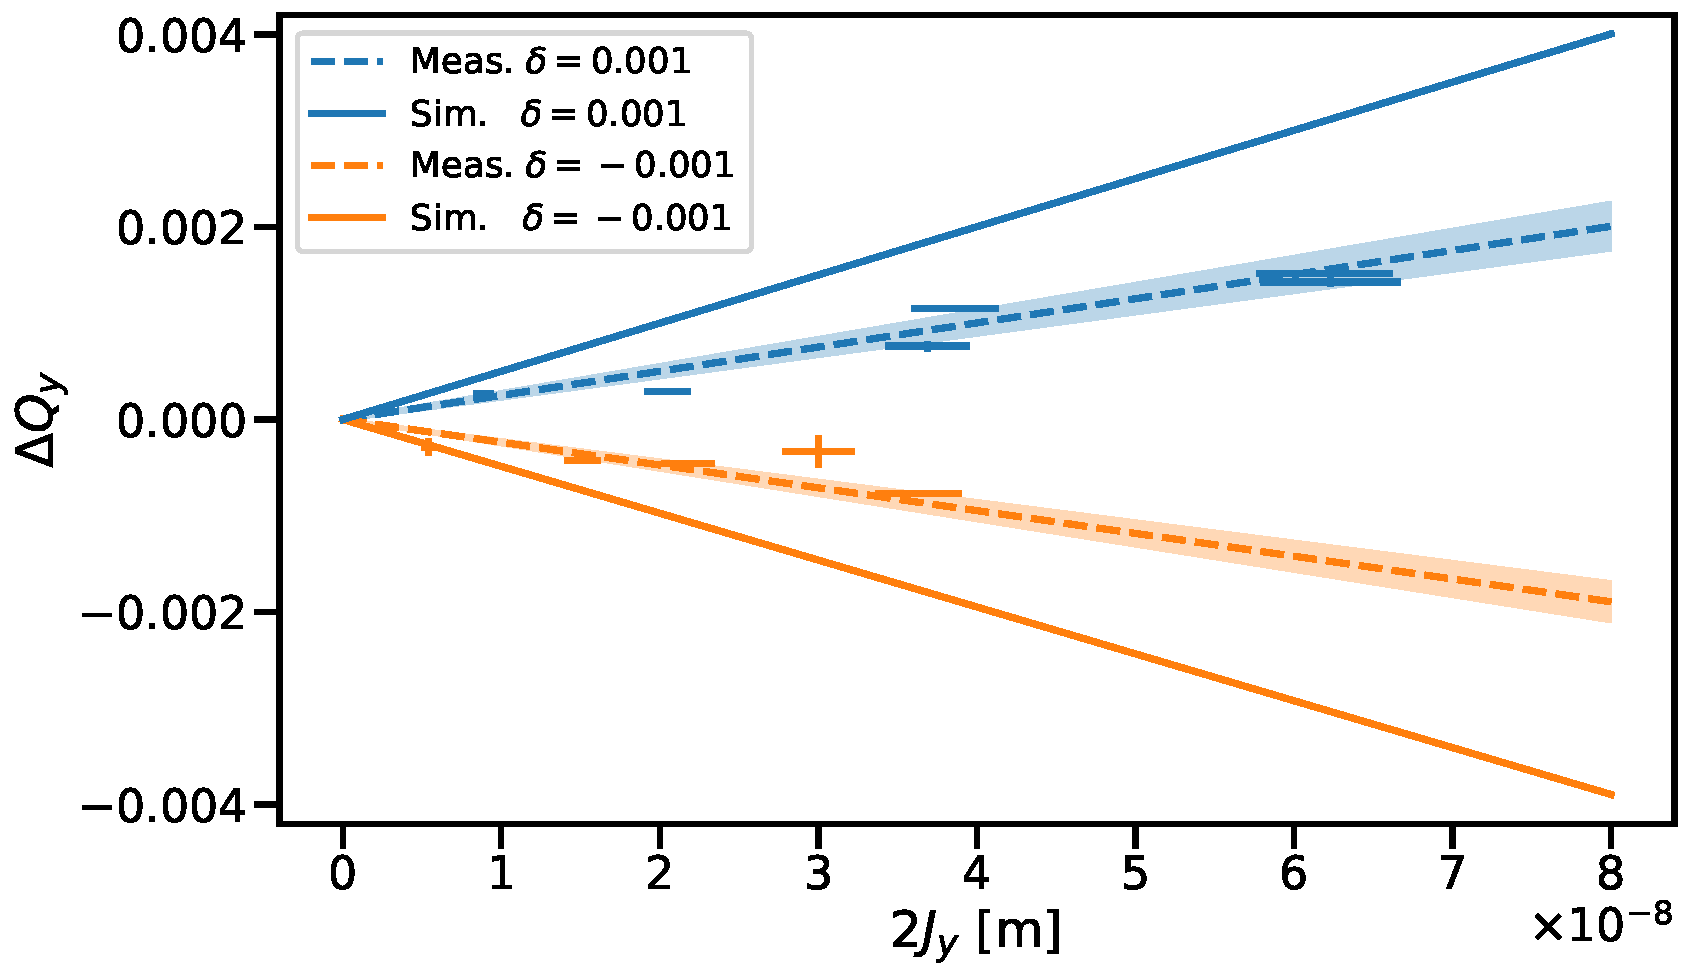
\includegraphics[width=\textwidth]{images/chromatic_amplitude_detuning/B2_Qyy_decay0.00.pdf}
      \caption{Vertical tune shift depending on the vertical action: 
      $\frac{\partial^2 Q_y}{\partial J_y \partial \delta}$.}
      \label{figure:decapoles:chromatic_amplitude_detuning:b2qyy}
  \end{subfigure}
  \caption{Measured and simulated tune shift due to a change of action via an AC-Dipole at two
  different momentum offsets. Each fit corresponds to a chromatic amplitude detuning term evaluated
  at a certain $\delta$.}
  \label{figure:decapoles:chromatic_amplitude_detuning:two_terms}
\end{figure}


\begin{table}[H]
  \centering
  \begin{tabular}{lrr}
  \toprule
   Type  & $\frac{\partial^2 Q_x}{\partial J_y \partial \delta}[10^{4}\mathrm{m}^{-1}]$ & $\frac{\partial^2 Q_y}{\partial J_y \partial \delta}[10^{4}\mathrm{m}^{-1}]$ \\
  \midrule
  $\delta = +0.001$ & & \\
  \hspace{2mm}Meas.  &   -1.16 ± 0.08 &   1.26 ± 0.15 \\
  \hspace{2mm}Sim.   &   -3.82 ± 0.01 &   2.47 ± 0.01 \\
  \hspace{2mm}Ratio  &    0.30 ± 0.02 &   0.51 ± 0.06 \\
  $\delta = -0.001$ & & \\
  \hspace{2mm}Meas.  &  1.47 ± 0.12  &  -1.18 ± 0.13 \\
  \hspace{2mm}Sim.   &  3.92 ± 0.01  &  -2.41 ± 0.01 \\
  \hspace{2mm}Ratio  &  0.38 ± 0.03  &   0.49 ± 0.05 \\
  \bottomrule
  \end{tabular}
  \caption{Comparison of the measured and simulated terms $\frac{\partial^2 Q_x}{\partial J_y
   \delta}$ and $\frac{\partial^2 Q_y}{\partial J_y \partial \delta}$ via PTC, at two
  discrete momentum offsets. Simulations include errors from normal sextupole to decahexapole and
  from skew octupole to decahexapole.}
  \label{table:decapoles:chromatic_ampdet}
\end{table}



A consistent difference between simulation and measurement is observed, which values and
ratios of measurement to model can be found in \cref{table:decapoles:chromatic_ampdet}.
The observed ratios of measurement to model for the chromatic amplitude detuning show slight
discrepancies compared to the bare chromaticity ones. These discrepancies could be due to the low
intensity kicks, which don't allow for a better fit. However, the similarity of the ratios suggests
an issue with the decapolar error model of the main dipoles, with measurements showing values about
half of those predicted by the magnetic model.


%==================================
%              Decay 
%==================================
%==================================
%              Decay 
%==================================
\section{Integrating Decay}



\begin{figure}[H]
    \centering
    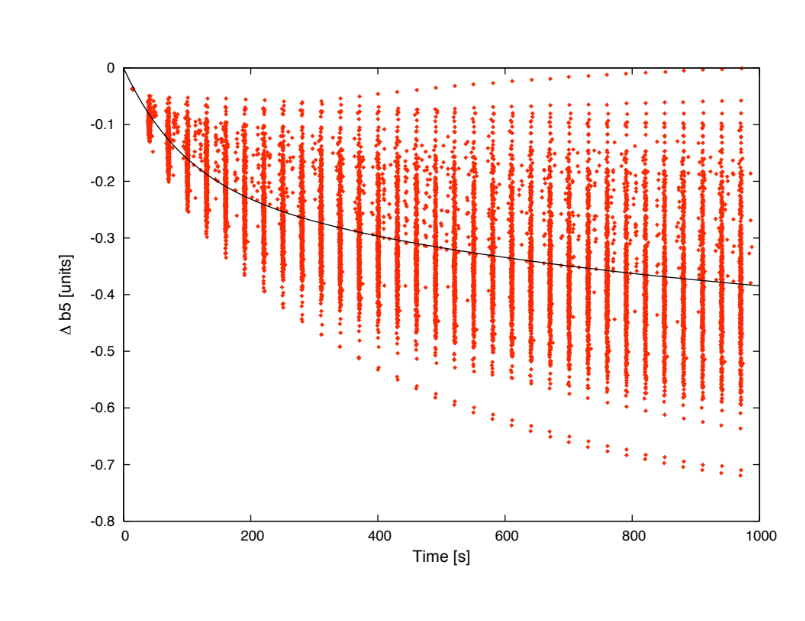
\includegraphics[width=\textwidth]{./images/decay_b5_mb.png}
    \caption{Decay of the integrated decapolar field in LHC's main dipoles at injection energy. The
    fit is shown in black~\cite{deniau_magnetic_2009}.}
    \label{fig:decapoles:decay_b5}
\end{figure}


%==================================
%      Resonance Driving Terms
%==================================
% === RDTs
\section{\todo{Resonance Driving Terms}}

Decapoles, due to their order, contribute to many RDTs. Indeed, 50 of them can be theoretically 
observed in simulations and measurements. In practice, the contributions of individual multipoles
become indistinguishable as many resonances or lines overlap, making it impossible to isolate
certain terms. Some resonances, described in~\cref{appendix:rdts}, are unique to certain multipoles
when considering no too high orders. Those resonances, provided that they are sufficiently strong
and the beam close to them, can be measured via their RDTs.

Of interest to the LHC Operation, is the RDT $f_{1004}$, driving the resonance $1Q_x - 4Q_y$.
It can be seen in the horizontal frequency spectrum at $-4Q_y$ with an amplitude dependence on
$J_y^2$. 
Figure~\cref{fig:decapoles:rdts:tune_diagram} shows a frequency
map~\cite{yannis_papaphilippou_detecting_nodate} of a simulation including decapolar field errors,
where their impact on the beam is easily noticeable. The \todo{red} particles evolving close to the
resonance are affected by it and are subject to large tune shifts. Eventually, those particles are 
lost when their amplitude becomes too large.

\begin{figure}[!htb]
    \centering
    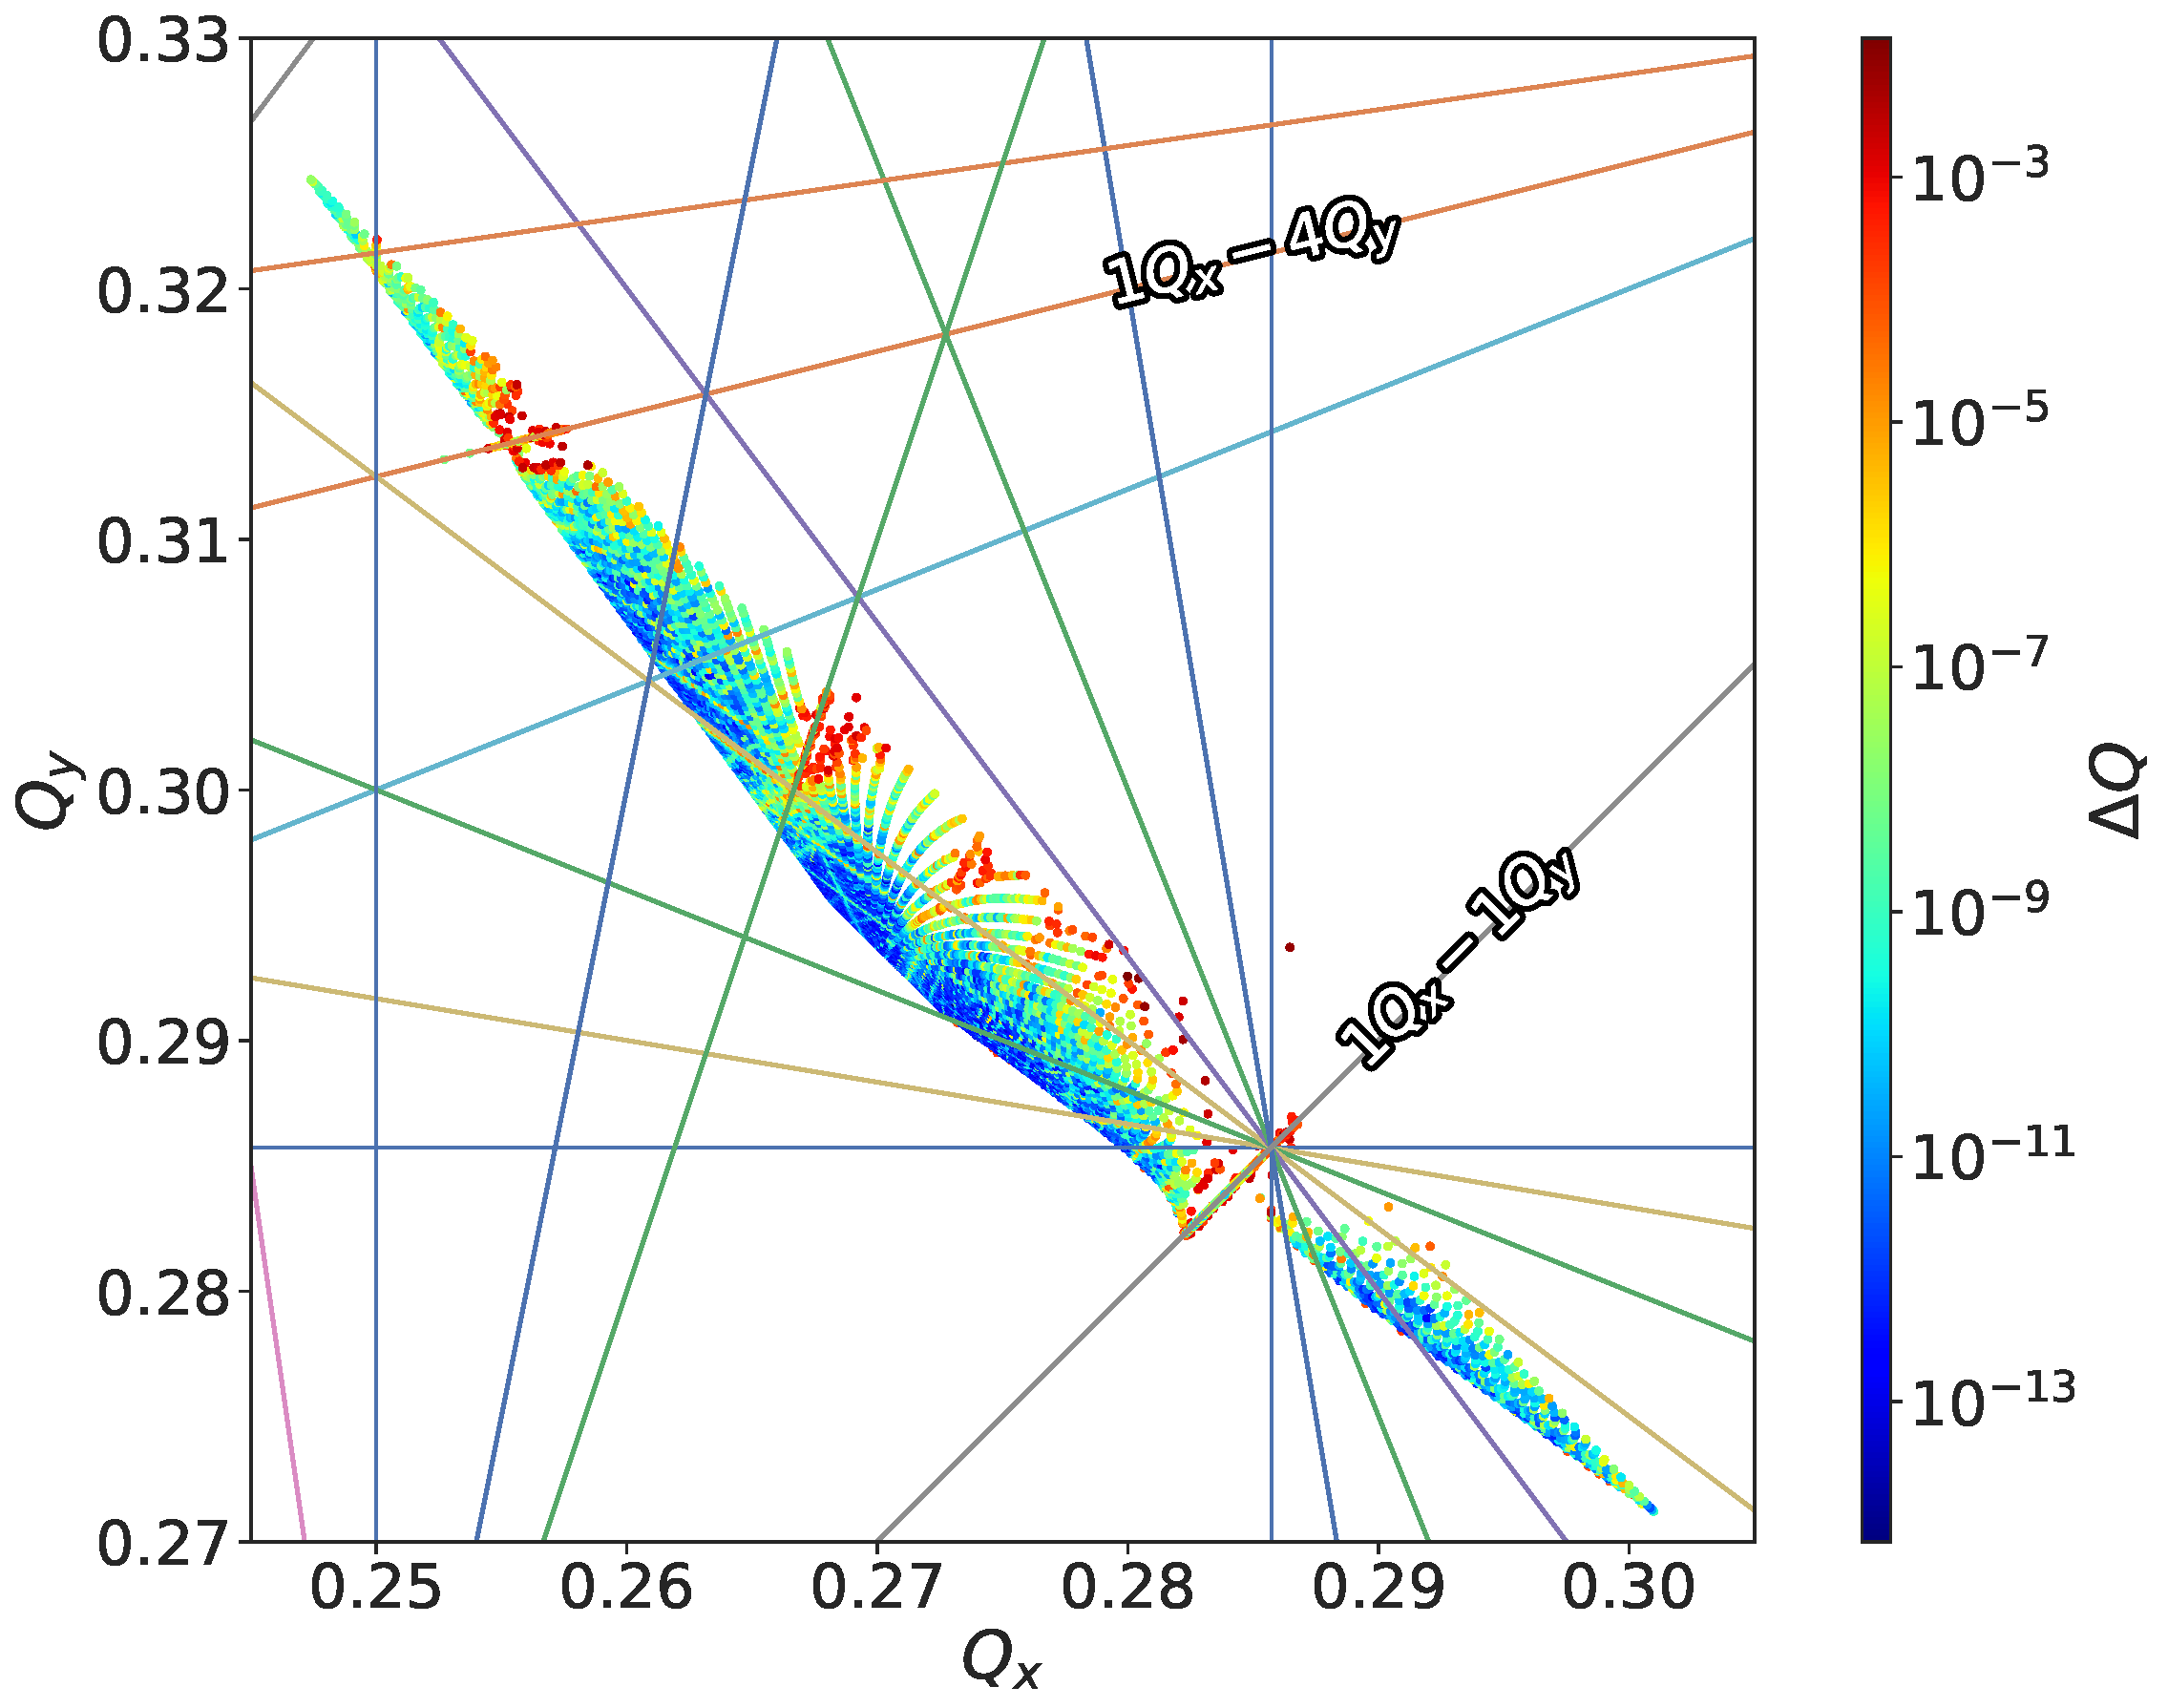
\includegraphics[width=0.8\textwidth]{./images/tune_diagram_f1004.pdf}
    \caption{Frequency map at injection energy, with decapolar field errors and nominal settings for
    landau octupoles. The highlighted resonance (1,-4), excited by decapoles, shows a degradation
    over 20,000 turns. The tune shift between the start and the end of the simulation is indicated
    in colour. \todo{change colormap}}
    \label{fig:decapoles:rdts:tune_diagram}
\end{figure}

Measuring turn-by-turn data without using any excitation is not a viable option as amplitudes are
not large enough. Spectral lines are indeed usually impossible to discern from the noise floor, 
making RDTs not measurable.
Measurements are hence taken with an AC-Dipole, introducing quadrupolar-like field errors in the 
linear regime~\cite{carlier_nonlinear_2020} and more complex effects in the non linear regime.
In practice, those effects are neglected. \textit{Forced} RDTs are measured with an
AC-Dipole and treated as \textit{free} as no compensation is applied.

Such forced measurements were taken for the first time in the LHC to observe the $f_{1004}$ RDT
at injection energy. The frequency line of the resonance $1Q_x - 4Q_y$ is seen at $4Q_y$ in the
horizontal spectrum, as shows \cref{fig:decapoles:rdts:spectrum_f1004}.

\begin{figure}[!htb]
    \centering
    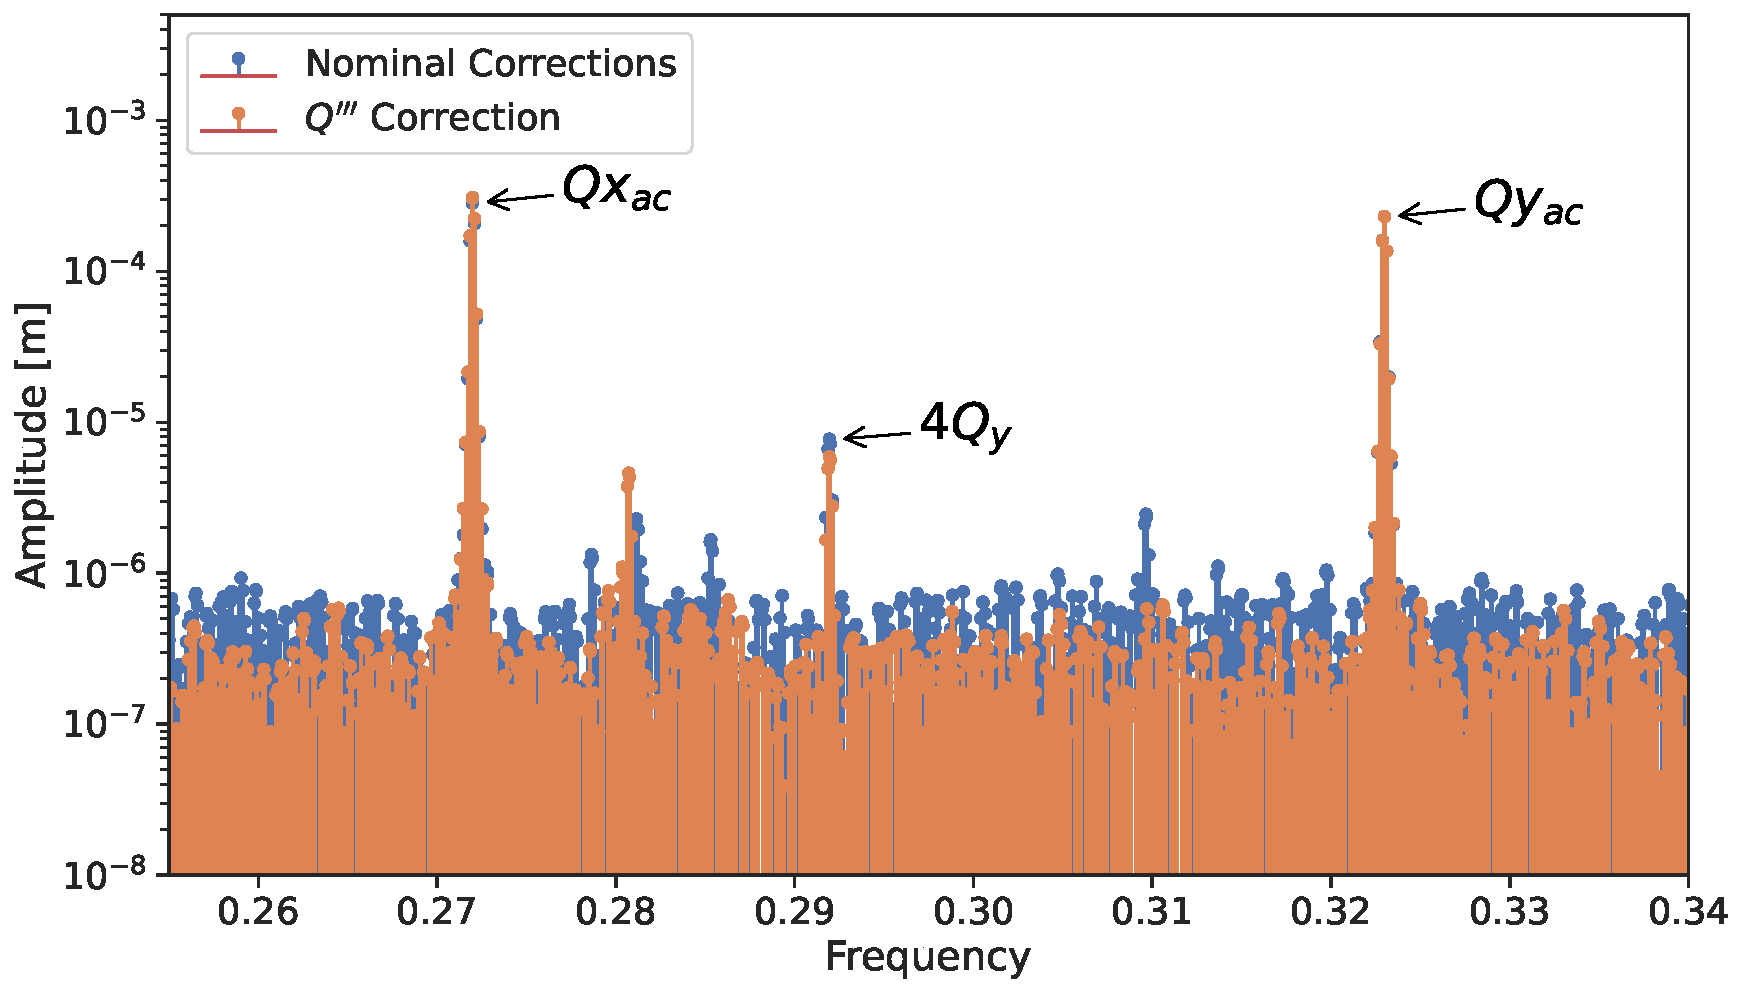
\includegraphics[width=0.9\textwidth]{./images/f1004x_spectrum.pdf}
    \caption{Horizontal frequency spectrum of turn-by-turn data, with nominal and beam-based
    corrections for the third order chromaticity $Q'''$. The $1Q_x - 4Q_y$ resonance can be seen
    at $-4Q_y$ with different amplitudes for each correction scheme.}
    \label{fig:decapoles:rdts:spectrum_f1004}
\end{figure}

%Moreover, \cref{fig:decapoles:rdts:spectrum_f1004} shows that the amplitude of this resonance line
%decreases upon application of beam-based corrections for $Q'''$. This translates to the amplitude
%of the RDT $f_{1004}$, as seen in \cref{fig:decapoles:rdts:f1004_dq3}.
%
%\begin{figure}[!htb]
%    \centering
%    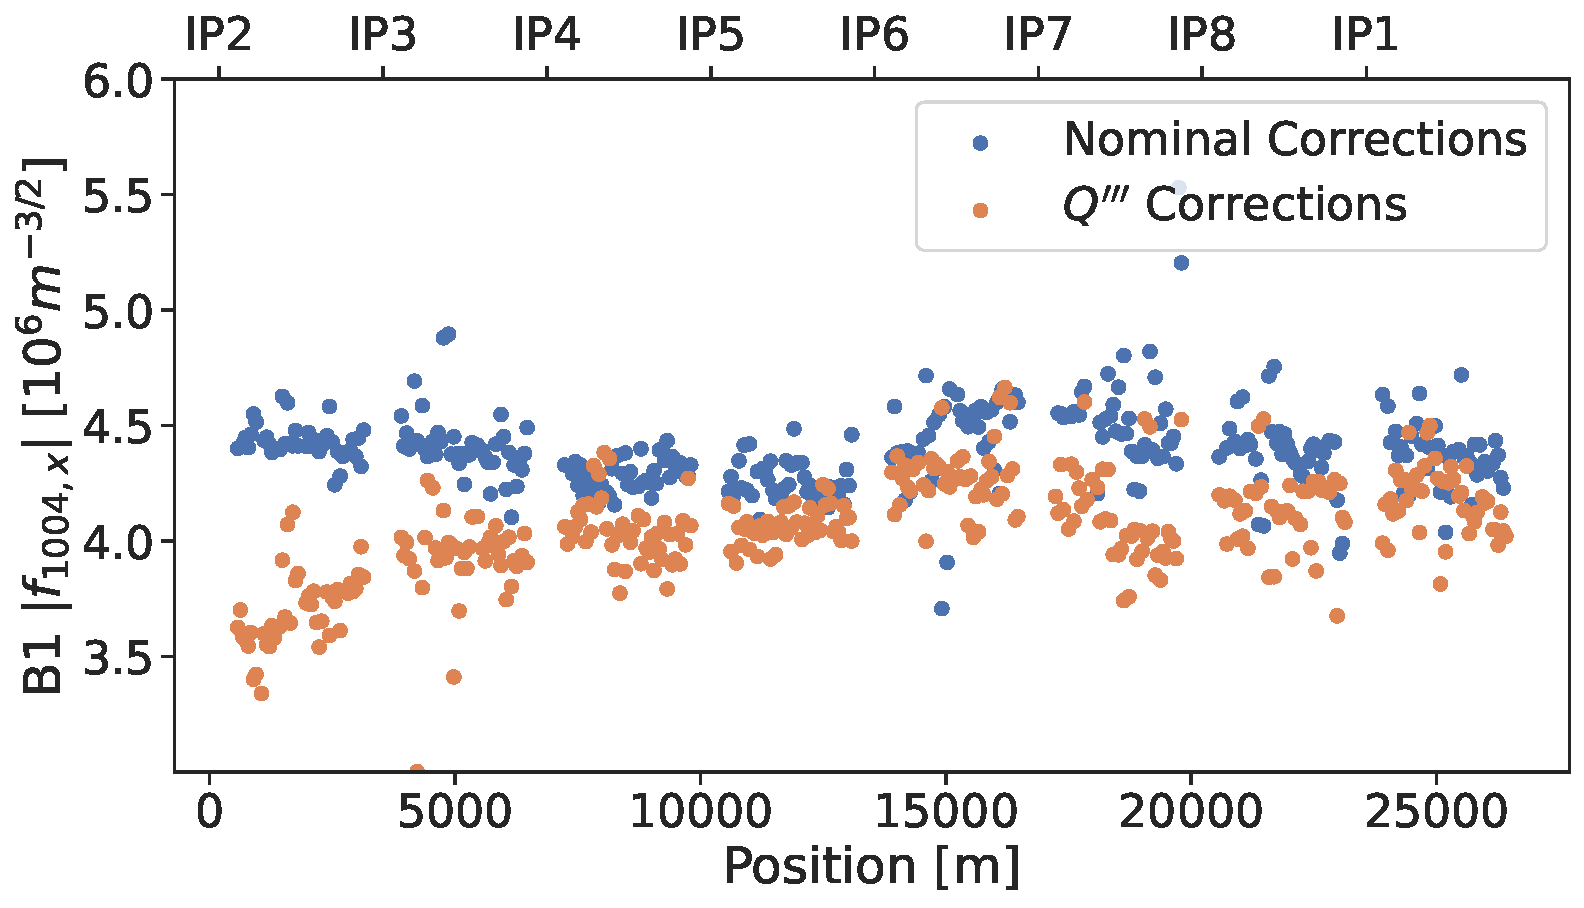
\includegraphics[width=0.9\textwidth]{./images/f1004_dq3.pdf}
%    \caption{Amplitude of the RDT $f_{1004}$ generated by normal decapoles, measured before and
%    after having applied beam-based corrections of the third order chromaticity $Q'''$.}
%    \label{fig:decapoles:rdts:f1004_dq3}
%\end{figure}

%\todo{
%    Measurements: \\
%    \begin{itemize}
%        \item 2022 Q'' and Q''' corrections 2022-04-24
%        \item 2022-10-19 Virgin machine
%        \item 2023-easter (FiDeL)
%        \item 2023-06-14 MD9549 (FiDeL and Q'''/ RDT corr)
%    \end{itemize}
%    Effect of RCO correction on RDT f1004 \\
%    Response
%}



% ---------------------------------------
%         Decapole Contribution
% ---------------------------------------
\subsection{\todo{Decapolar Contribution}}
\label{section:decapoles:decapolar_contribution_correction}

Decapolar fields are the main contributors to the RDT $f_{1004}$. As such, powering the decapolar
correctors is a good way to correct the related resonances.
Being linear with the strength of the correctors, the RDT can be corrected via a response matrix.

Measurements were taken in order to attempt such a correction and get a baseline for the amplitude
of the RDT without decapolar correctors and with the nominal FiDeL corrections applied.
Corrections were made on the base of those nominal settings and applied on top. The strength of the
decapolar correctors is shown in \cref{tab:decapoles:rdts:correction_f1004_k5} for the FiDeL
settings, the delta applied on top and the final correction values.


\begin{table}[!htb]
    \centering
    \begin{tabular}{lrrr}
    \toprule
    Circuit & FiDeL $K_5 [\textrm{m}^{-5}]$ & $\Delta K_5 [\textrm{m}^{-5}]$ & $K_5 [\textrm{m}^{-5}]$\\
    \midrule
    Beam 1 & \\
    \hspace{2mm}RCD.A12B1 &$-4582$ & $6055 $ &  $ 1473 $\\
    \hspace{2mm}RCD.A23B1 &$-5106$ & $7    $ &  $-5099 $\\
    \hspace{2mm}RCD.A34B1 &$-4855$ & $3827 $ &  $-1028 $\\
    \hspace{2mm}RCD.A45B1 &$-4577$ & $-4746$ &  $-9323 $\\
    \hspace{2mm}RCD.A56B1 &$-4125$ & $-4903$ &  $-9028 $\\
    \hspace{2mm}RCD.A67B1 &$-5166$ & $2961 $ &  $-2205 $\\
    \hspace{2mm}RCD.A78B1 &$-6827$ & $3593 $ &  $-3234 $\\
    \hspace{2mm}RCD.A81B1 &$-5500$ & $2380 $ &  $-3120 $\\
    \hspace{2mm}Total     &$-40738$& $9174 $ &  $-31564$\\
    Beam 2 & \\  % inverted the signs of the correction
    \hspace{2mm}RCD.A12B2 &$-4490$ & $3639 $ &  $-851  $\\
    \hspace{2mm}RCD.A23B2 &$-5155$ & $-1147$ &  $-6302 $\\
    \hspace{2mm}RCD.A34B2 &$-4825$ & $-1038$ &  $-5863 $\\
    \hspace{2mm}RCD.A45B2 &$-4619$ & $3986 $ &  $-633  $\\
    \hspace{2mm}RCD.A56B2 &$-4064$ & $2944 $ &  $-1120 $\\
    \hspace{2mm}RCD.A67B2 &$-5066$ & $2357 $ &  $-2709 $\\
    \hspace{2mm}RCD.A78B2 &$-6866$ & $-2952$ &  $-9818 $\\
    \hspace{2mm}RCD.A81B2 &$-5446$ & $1825 $ &  $-3621 $\\
    \hspace{2mm}Total     &$-40531$& $9614 $ &  $-30917$      \\
    \bottomrule
    \end{tabular}
    \caption{Strength of decapolar correctors with nominal FiDeL settings and after application of
    corrections aiming at reducing both the RDT $f_{1004}$ and $Q'''$. The total value as a direct
    incidence on the chromaticity}
    \label{tab:decapoles:rdts:correction_f1004_k5}
\end{table}

This RDT correction also serves as a partial $Q'''$ correction. To fully correct $Q'''$ indeed
approximately requires a strength of $+13,000 K_5$ distributed amongst the correctors. Therefore,
this new approach reduces $Q'''$ by about $70\%$ compared to the previous method. The chromatic
amplitude detuning terms are also expected to be decreased.
Result of those measurements, as well as the inverse of the correction, are shown in 
\cref{fig:decapoles:rdts:f1004_correction_B2}

\begin{figure}[!h]
    \centering
    \begin{subfigure}{1\textwidth}
        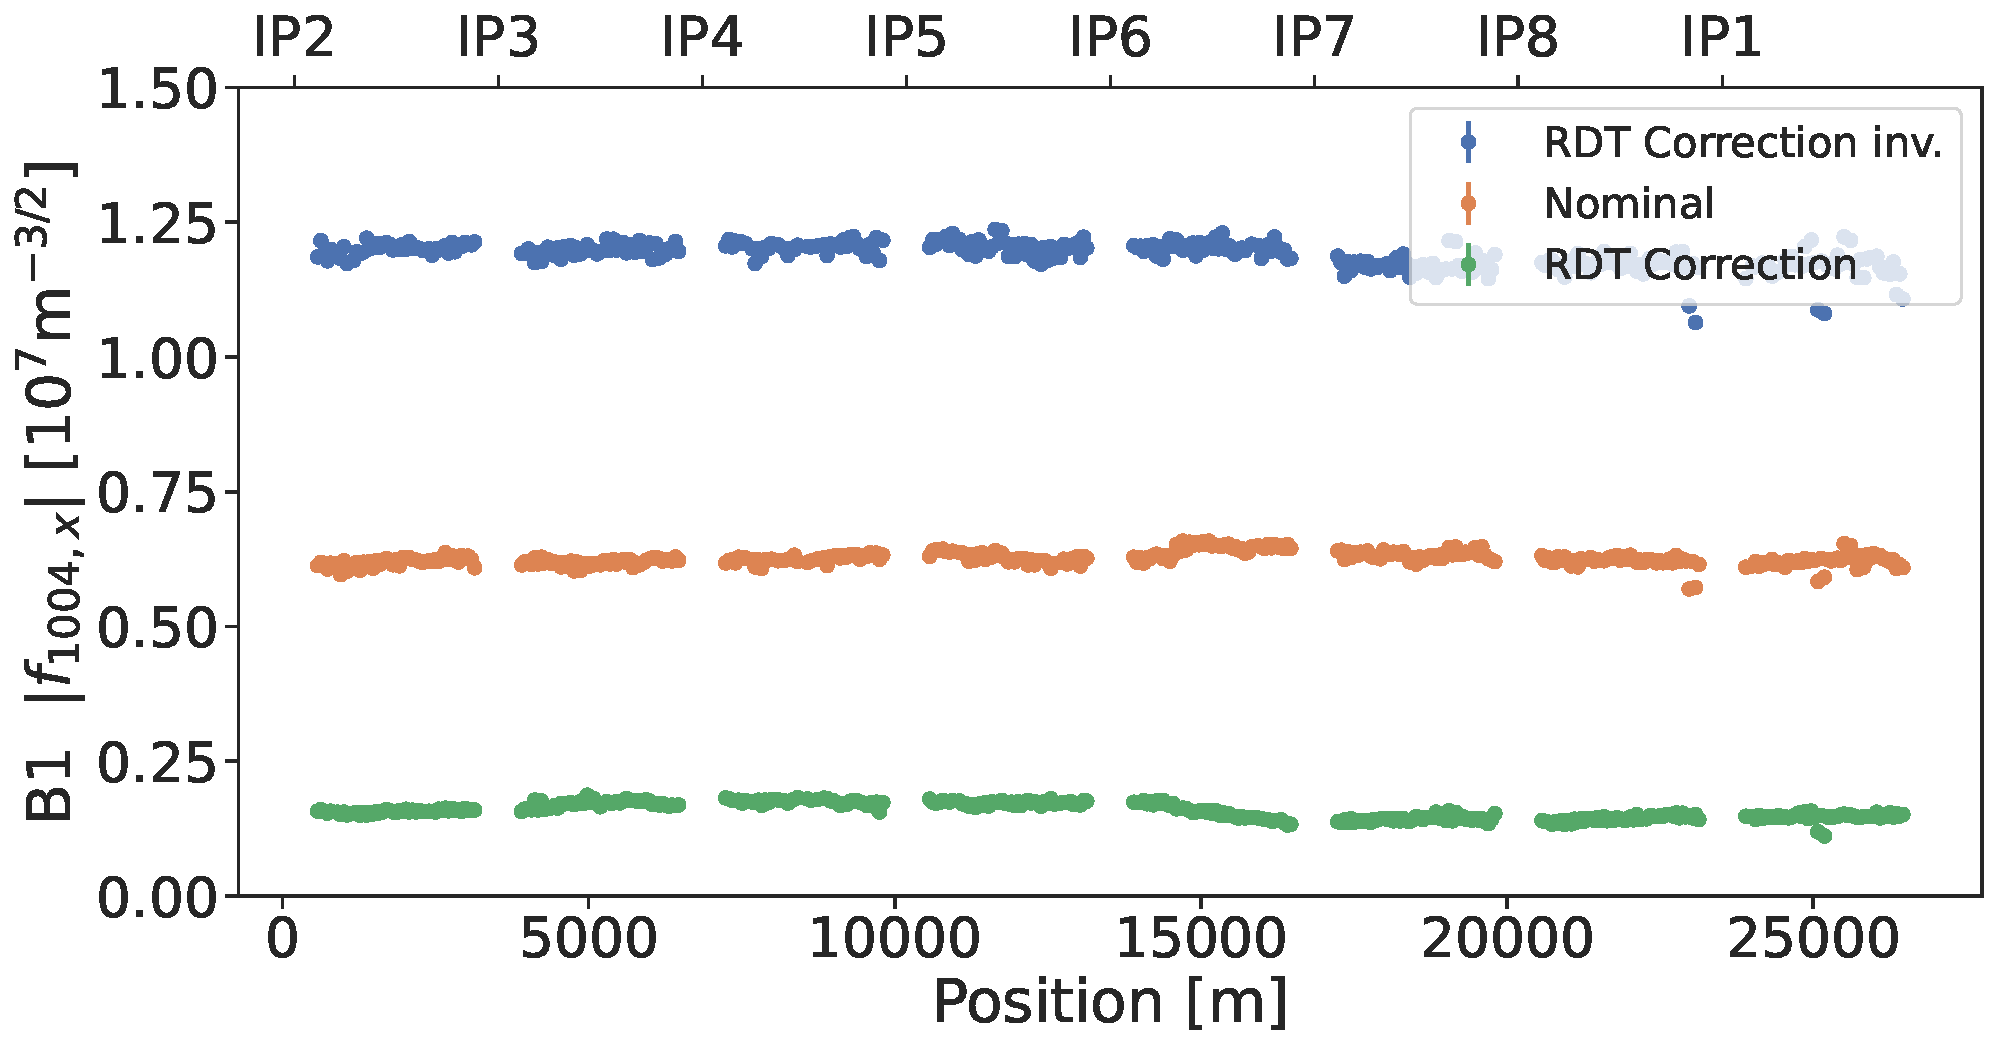
\includegraphics[width=0.9\textwidth]{./images/f1004/f1004x_corrections_B1.pdf}
        \caption{$|f_{1004}|$ for Beam 1}
        \vspace{0.5cm}
    \end{subfigure}
    \begin{subfigure}{1\textwidth}
        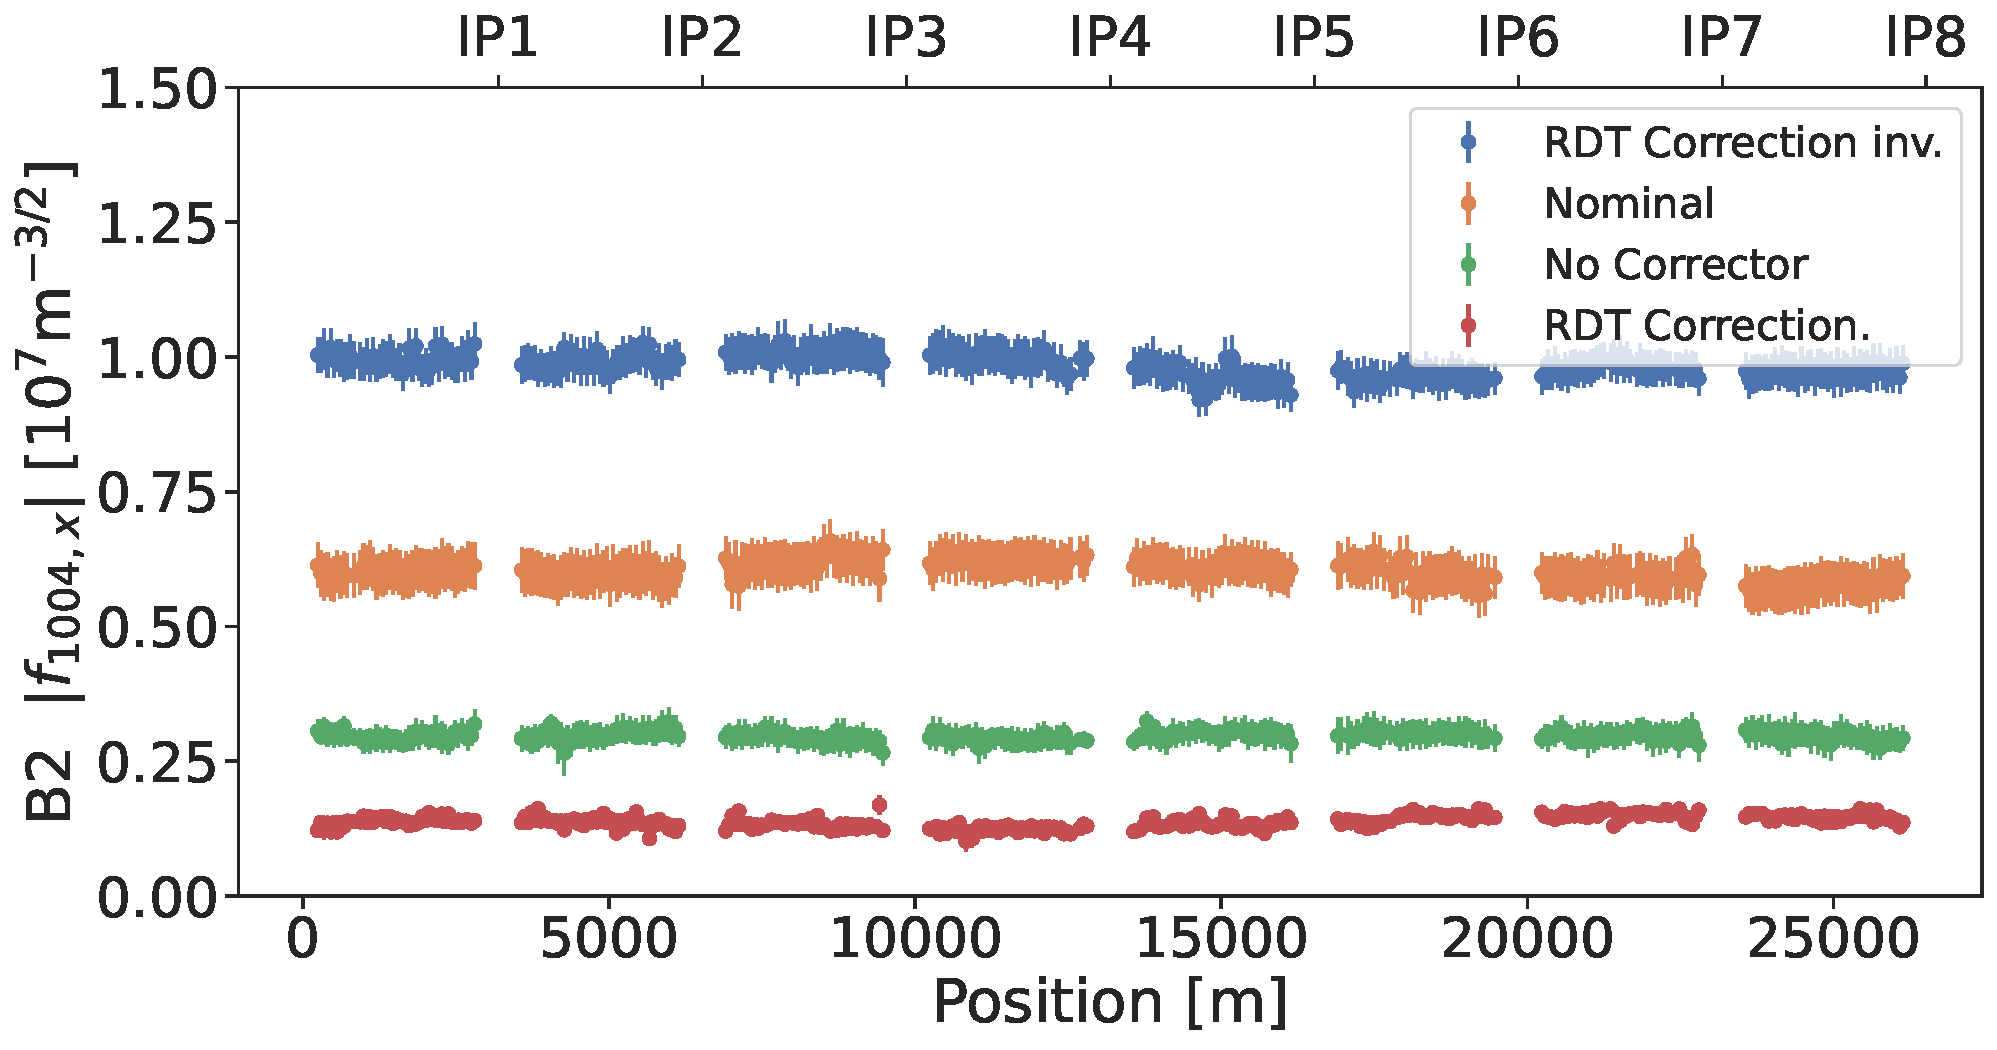
\includegraphics[width=0.9\textwidth]{./images/f1004/f1004x_corrections_B2.pdf}
        \caption{$|f_{1004}|$ for Beam 2}
    \end{subfigure}
    \caption{Measured $f_{1004}$ with decapolar correctors powered off, nominal settings, and
    combined RDT \& $Q'''$ correction with normal and opposite signs.}
    \label{fig:decapoles:rdts:f1004_correction_B2}
\end{figure}


Although the FiDeL scheme was not intended to correct the RDT but rather only $Q'''$, it would be 
expected for it to lower the amplitude of the RDT. It can though be seen that it degrades the
resonance compared to the machine with no decapolar correctors. On the other hand, the newly
computed RDT correction does lower the amplitude of $f_{1004}$ as expected.  Its inverse has the
opposite effect.

Simulations were run with decapolar correctors turned of and with the absolute value of the RDT
correction. The response of the RDT between those two schemes is shown in 
\cref{fig:decapoles:rdt:b1_response_corr}. The difference between their RMS value ratio is $\approx
6\%$, indicating that simulations correctly model the decapolar correctors.

\begin{figure}[!htb]
    \centering
    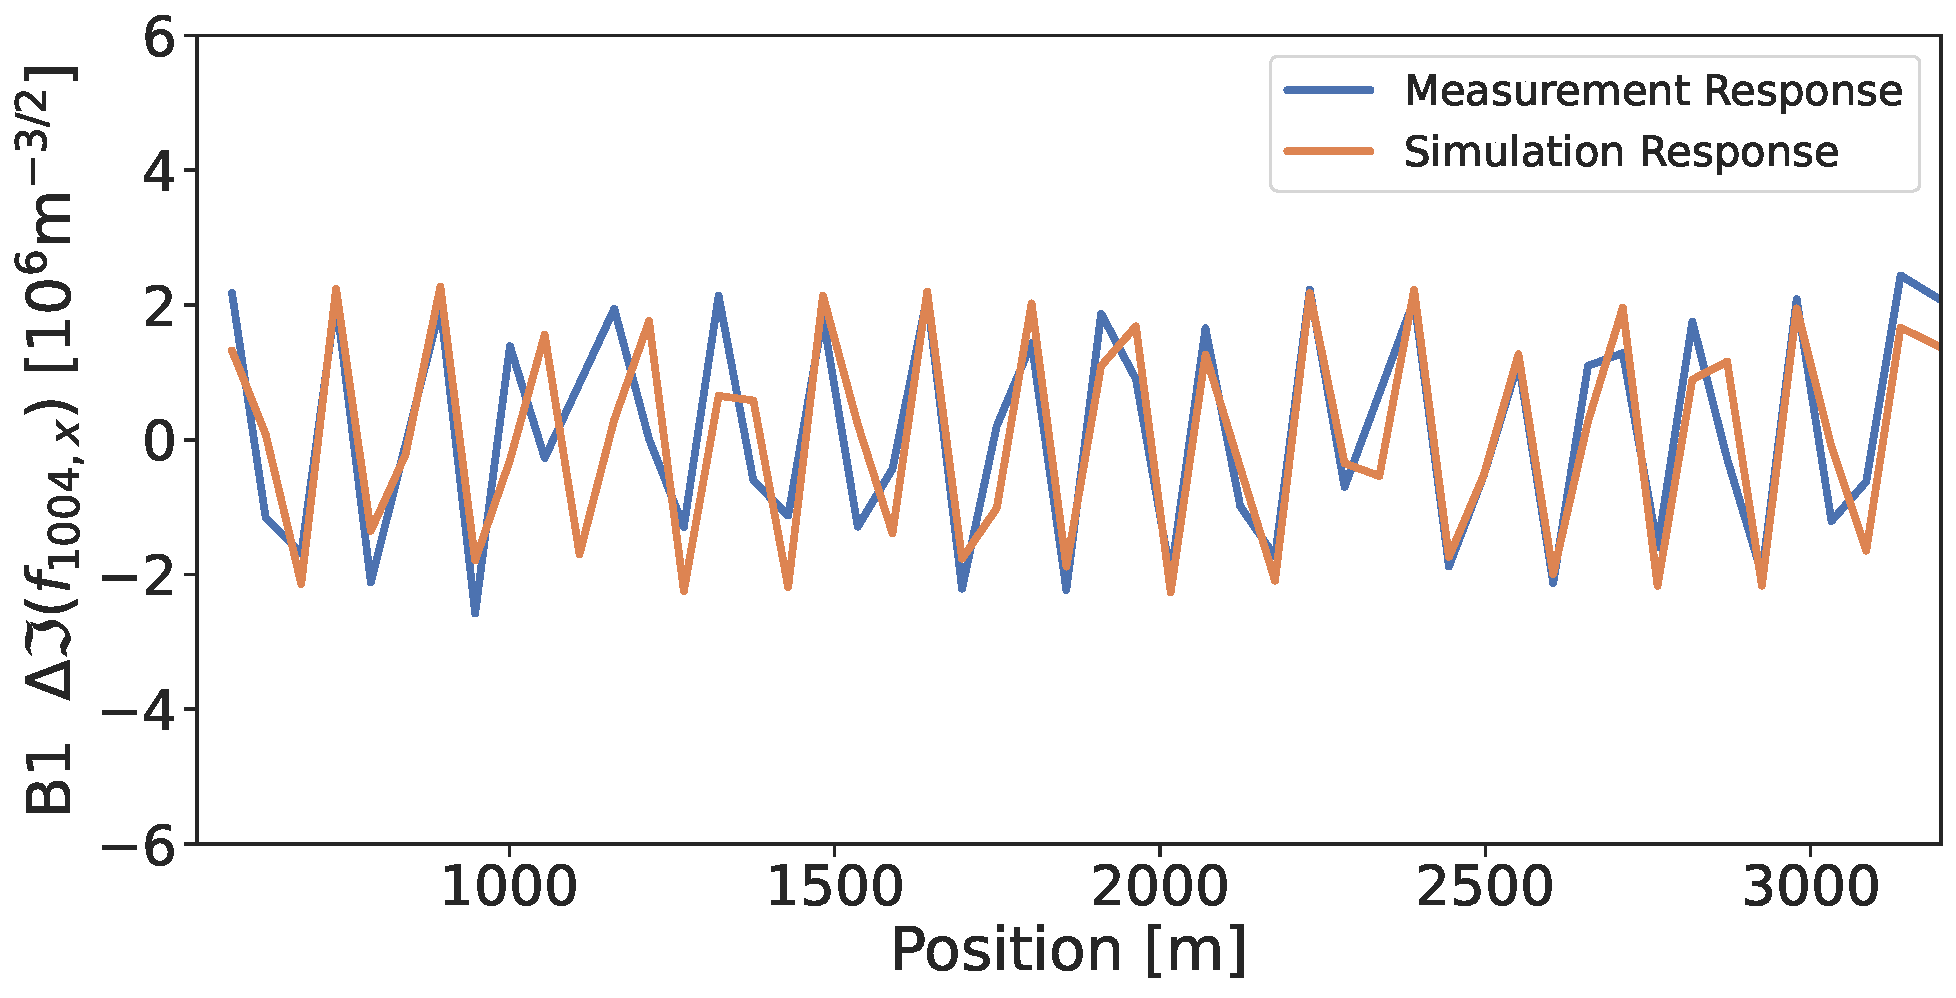
\includegraphics[width=0.9\textwidth]{./images/f1004/b1_response_rdt_corr.pdf}
    \caption{Comparison for measurement and simulation of the response of the imaginary part of
    $f_{1004}$ upon application on unpowered correctors of the RDT corrections.}
    \label{fig:decapoles:rdt:b1_response_corr}
\end{figure}


% ---------------------------------------
%        Higher Order Contribution
% ---------------------------------------
\subsection{\review{Higher Order Contributions}}

% Measurements in 
% /afs/cern.ch/work/m/mlegarr2/public/beta_beat_output/2024-05-21

To produce collisions at top energy, \textit{crossing angles} are introduced via the orbit
correctors located in the triplets, before the separation dipoles and the matching section of the
interaction regions (\texttt{MCBX}, \texttt{MCBY} and \texttt{MCBC})~\cite{de_maria_lhc_2008}. Those
collisions happen with a small $\beta*$, currently 30cm, requiring strong quadrupolar fields from
the triplets.

At such $\beta$, those triplets also generate strong dodecapolar field errors. Because of the
crossing-angles, feed-down appears and lower-order fields can be observed.
Such feed-down to decapolar fields was observed during the first commissioning of Run~3, in
2022~\cite{maclean_prospects_2022}.
\cref{fig:decapoles:f1004_from_feeddown} shows how the RDT $f_{1004}$, normally affected by
decapoles, varies with the application of crossing angles.

\begin{figure}[!htb]
    \centering
    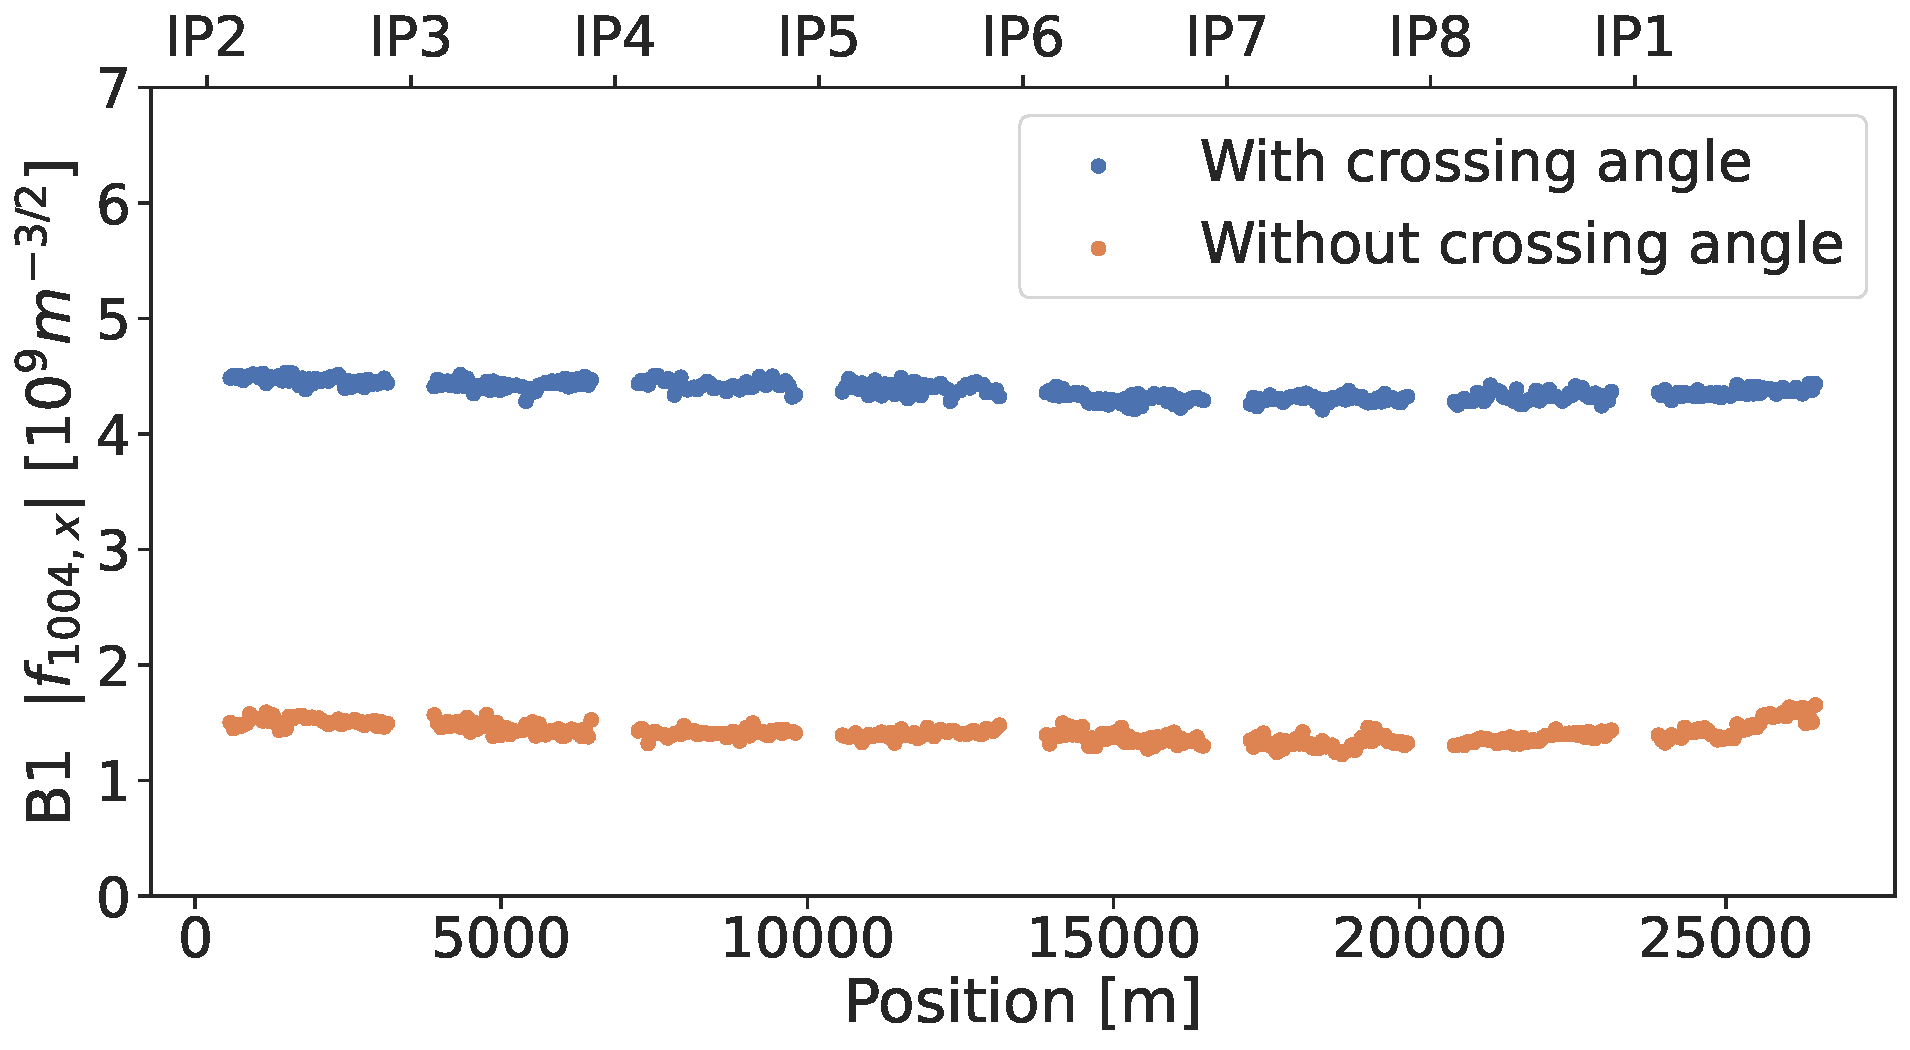
\includegraphics[width=0.9\textwidth]{./images/f1004x_feed-down_b6_triplets.pdf}
    \caption{Varying amplitude of the decapolar RDT $f_{1004}$ depending on the activation or not of
    the crossing angle at the IP. Offsets in orbit create feed-down from higher orders.}
    \label{fig:decapoles:f1004_from_feeddown}
\end{figure}

Such a contribution is though not expected at injection energy, as the triplets aren't powered as
much as at top energy, $\beta*$ being set at around $10$m.

% ---------------------------------------
%        Lower Order Contribution
% ---------------------------------------
\subsection{\review{Lower Order Contributions}}

% http://localhost:8888/lab/workspaces/auto-d/tree/work_afs2/jupyter/resonance_driving_terms/measurements/2024-03-13_b3_b4_effect_on_b5/Sextupoles_and_Octupoles.ipynb

% ------- Introduction
\subsubsection{\review{First Observation}}

As described in \cref{appendix:transfer_maps}, multipoles can combine to create fields that are seen
as higher orders when considering higher orders of the BCH expansion.
For decapoles, combinations of several sextupoles and sextupoles with octupoles give rise to
decapolar-like fields, as described in
\cref{table:appendix:transfer_maps:bch_resulting_orders_combination}. The following parts of this
section will describe those combinations.

This effect was observed in 2022 during Run 3's commissioning. New corrections of the non-linear
chromaticity $Q''$ and $Q'''$ were performed, and RDT measurements taken before and after their
correction. As $Q'''$ was corrected, the expectation was that the RDT $f_{1004}$ would also lower
with the reduction of the decapolar strengths $K_5$. However, an increase of the RDT was observed,
as shows \cref{fig:decapoles:f1004_dq2_dq3}.

\begin{figure}[H]
    \centering
    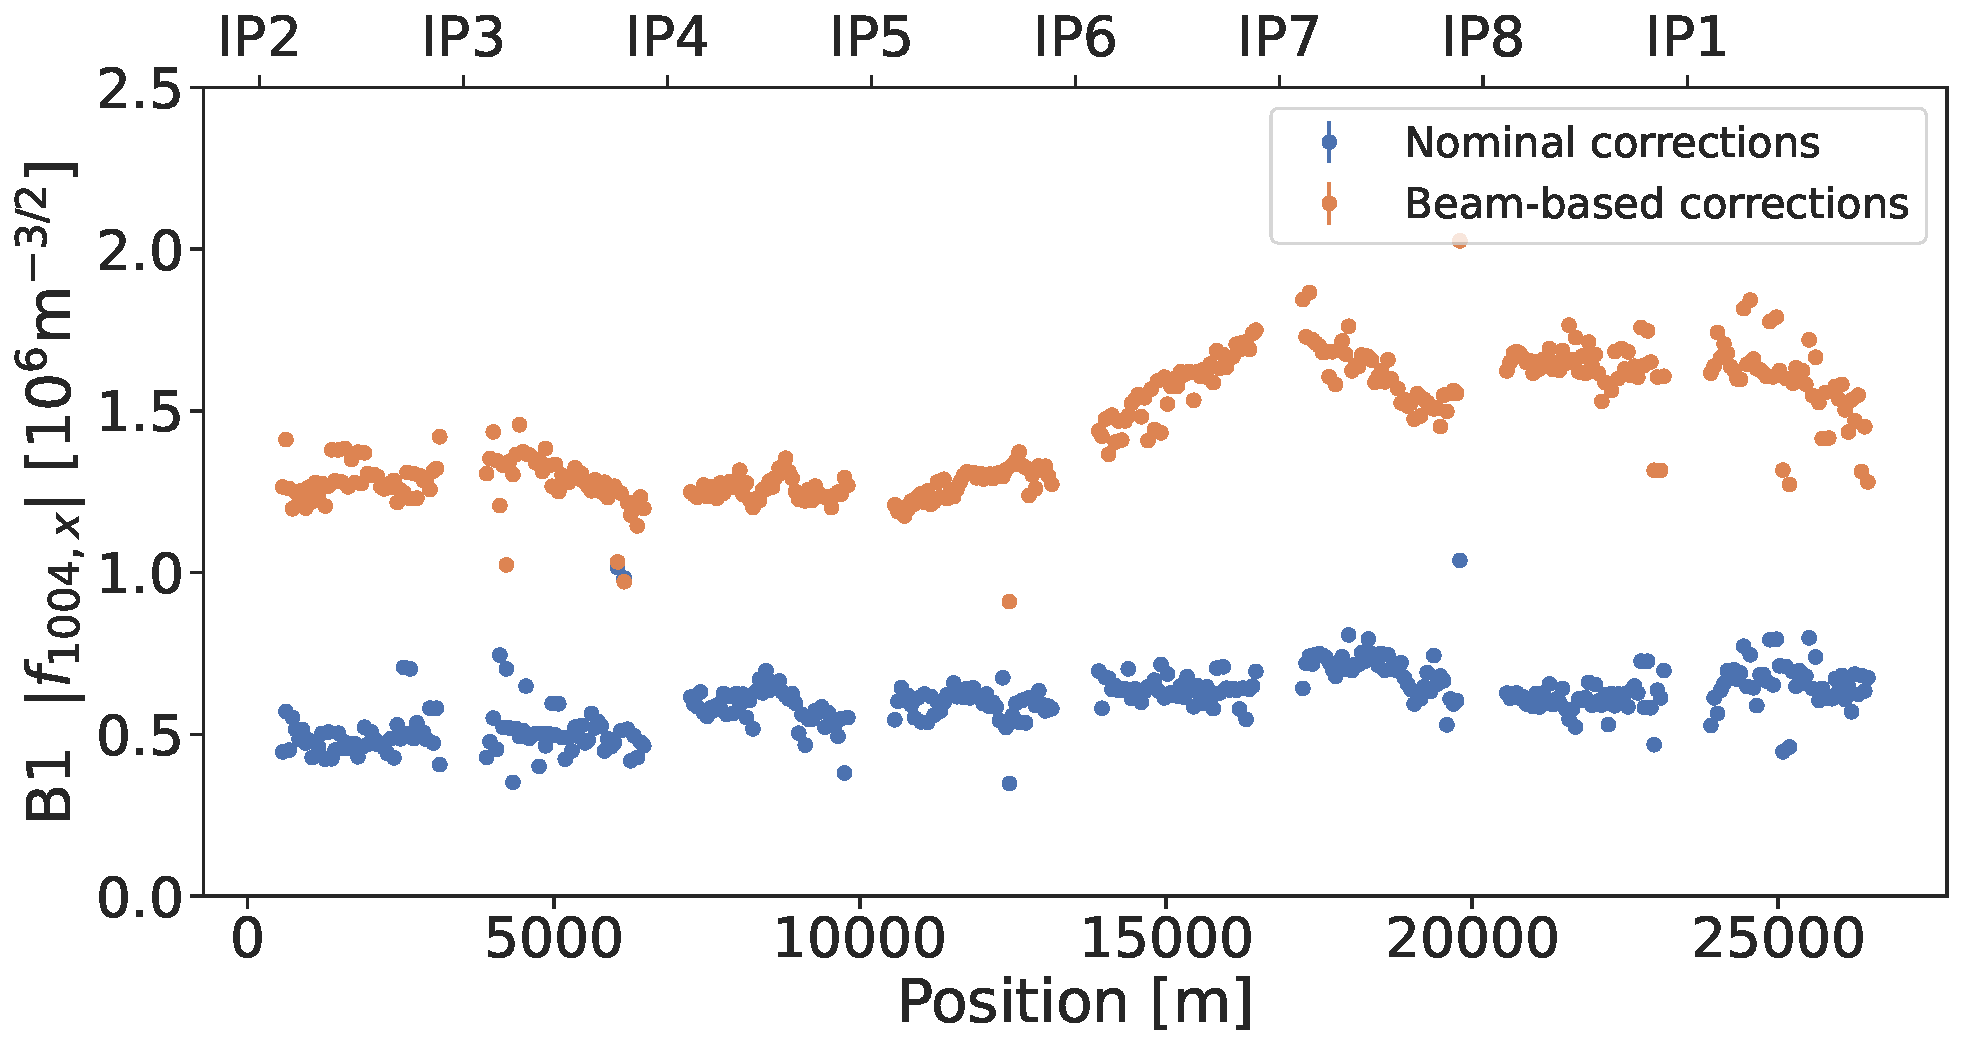
\includegraphics[width=0.9\textwidth]{./images/f1004_dq2_dq3_2022.pdf}    
    \caption{Non intuitive increase of the RDT $f_{1004}$ after application of both the $Q''$ and
    $Q'''$ corrections.\todo{redo plot}}
    \label{fig:decapoles:f1004_dq2_dq3}
\end{figure}


% ------- Action dependance
\subsubsection{\review{Action Dependance and Analysis}}

Resonance lines in the frequency spectrum are often contributed to by several multipoles. Some lines
start getting a contribution with rather high multipole orders, like the RDT $f_{1004}$ considered
here. The line $4Q_y$ in the horizontal spectrum is indeed contributed to by decapoles and then only
by decatetrapoles. When the main contributing field alone is varied, it is easy to reconstruct the
RDT, as its fit is only dependant its action dependance ($\propto J_x^{*} J_y^{*}$). Several
turn-by-turn measurements at the same configuration can be taken wit varying kick amplitudes,
refining the RDT value with more data points for the fit.

Considering the contribution of lower order multipoles is a bit trickier, as the second order RDTs
change the dependance of the frequency line~\cite{franchi_first_2014}. In order to be able to
compare the RDT from several turn by turn measurements, the same kick amplitude must then be used.
Failing to do so would lead to a poor fit of the line amplitude relative to the action, resulting in
an RDT with incorrect amplitude and significant noise.

%\todo{simulation plot of varying amplitudes for Q' = 2 and noise created from it}


% ------- Sextupoles ----------
\subsubsection{\review{Sextupoles}}

At the third order of the BCH expansion, the combination of two sextupoles yields a decapolar-like
expression. This means that, during normal operation of the machine, decapolar observables will be
altered when adjusting parameters such as the linear chromaticity $Q'$. 
Derivation of such a combination can be found in \cref{appendix:transfer_map:two_sextupoles}. The
resulting Hamiltonian indeed is similar to the terms of a decapole, dropping the $p_{x,y}$ terms for
readability:

\begin{equation}
    \begin{aligned}
         (H_3)^3 &\propto \frac{1}{48} \left(x^5 - 2x^3y^2 - 3xy^4 \right)\\
                 &\sim    x^5 - 10x^3y^2 + 5xy^4.
    \end{aligned}
    \label{eq:decapoles:sextupoles_b5}
\end{equation}

To quantify the actual impact of such an equation on the LHC, a simulation was run with injection
optics while varying this same linear chromaticity $Q'$. No higher fields than sextupoles are 
have been included, including field errors. The resulting effect on the RDT $f_{1004}$
can be seen in \cref{fig:decapoles:rdts:simulated_f1004_from_sextupoles}.

\begin{figure}[H]
    \centering
    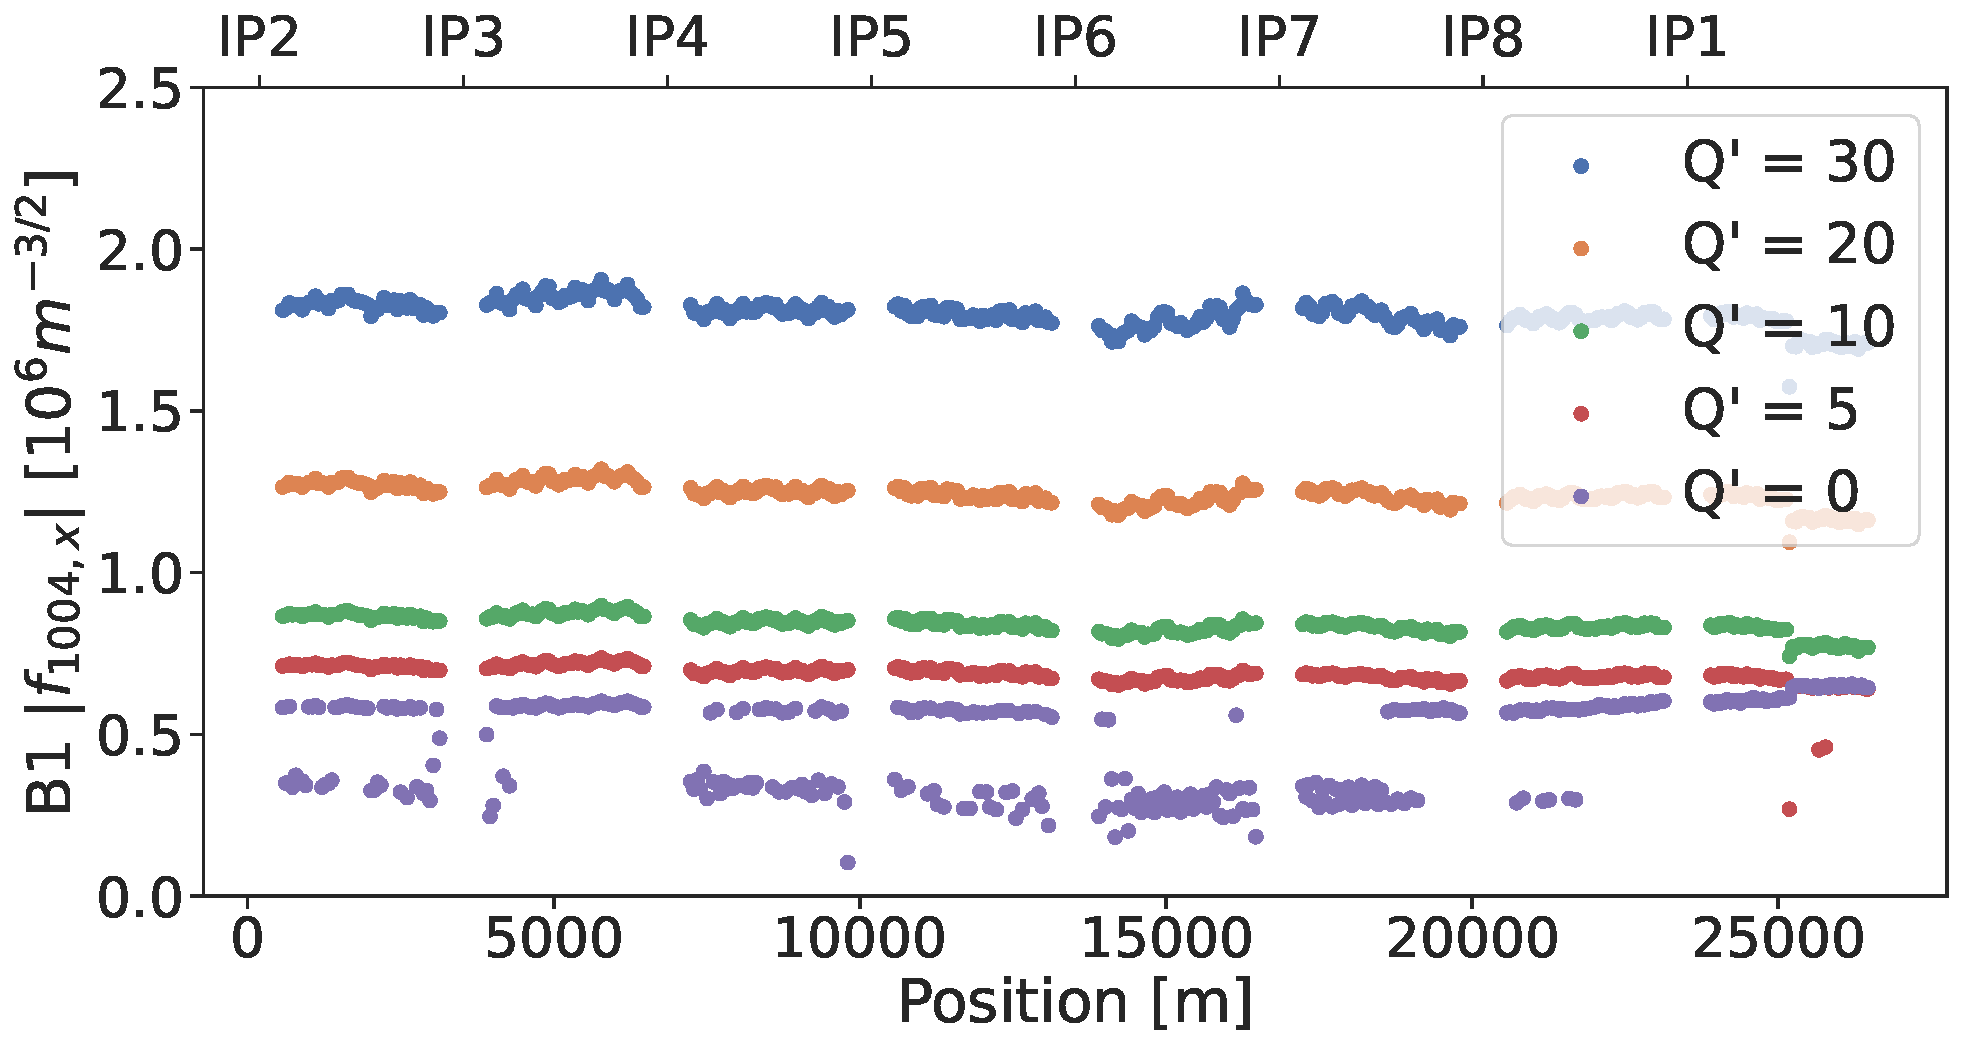
\includegraphics[width=0.7\textwidth]{./images/f1004/f1004_dq.pdf}
    \caption{Simulated change of the decapolar RDT $f_{1004}$ with varying linear
    chromaticity $Q'$ generated by sextupoles. The combination of sextupolar fields clearly shows a 
    increase in decapolar RDT.}
    \label{fig:decapoles:rdts:simulated_f1004_from_sextupoles}
\end{figure}

As the linear chromaticity increases, the overall $K_3$ strength of sextupoles actually becomes 
more negative. Considering the previous \cref{eq:decapoles:sextupoles_b5}, a higher chromaticity
is expected to increase the amplitude of the RDT $f_{1004}$, related to the last term $xy^4$.
\cref{fig:decapoles:sextupoles_k3_f1004} shows how the RDT is expected to vary, depending on the
overall sextupoles strength and the linear chromaticity. It can be noted that although the relation
between $K_3$ and $Q'$ is linear, that of $K_3$ and the RDT varies with the cubed strength. Using 
the sum of the cubed strength is possible due to the chromaticity knob being a factor applied on all
sextupoles at the same time.

\begin{figure}[!htb]
    \centering
    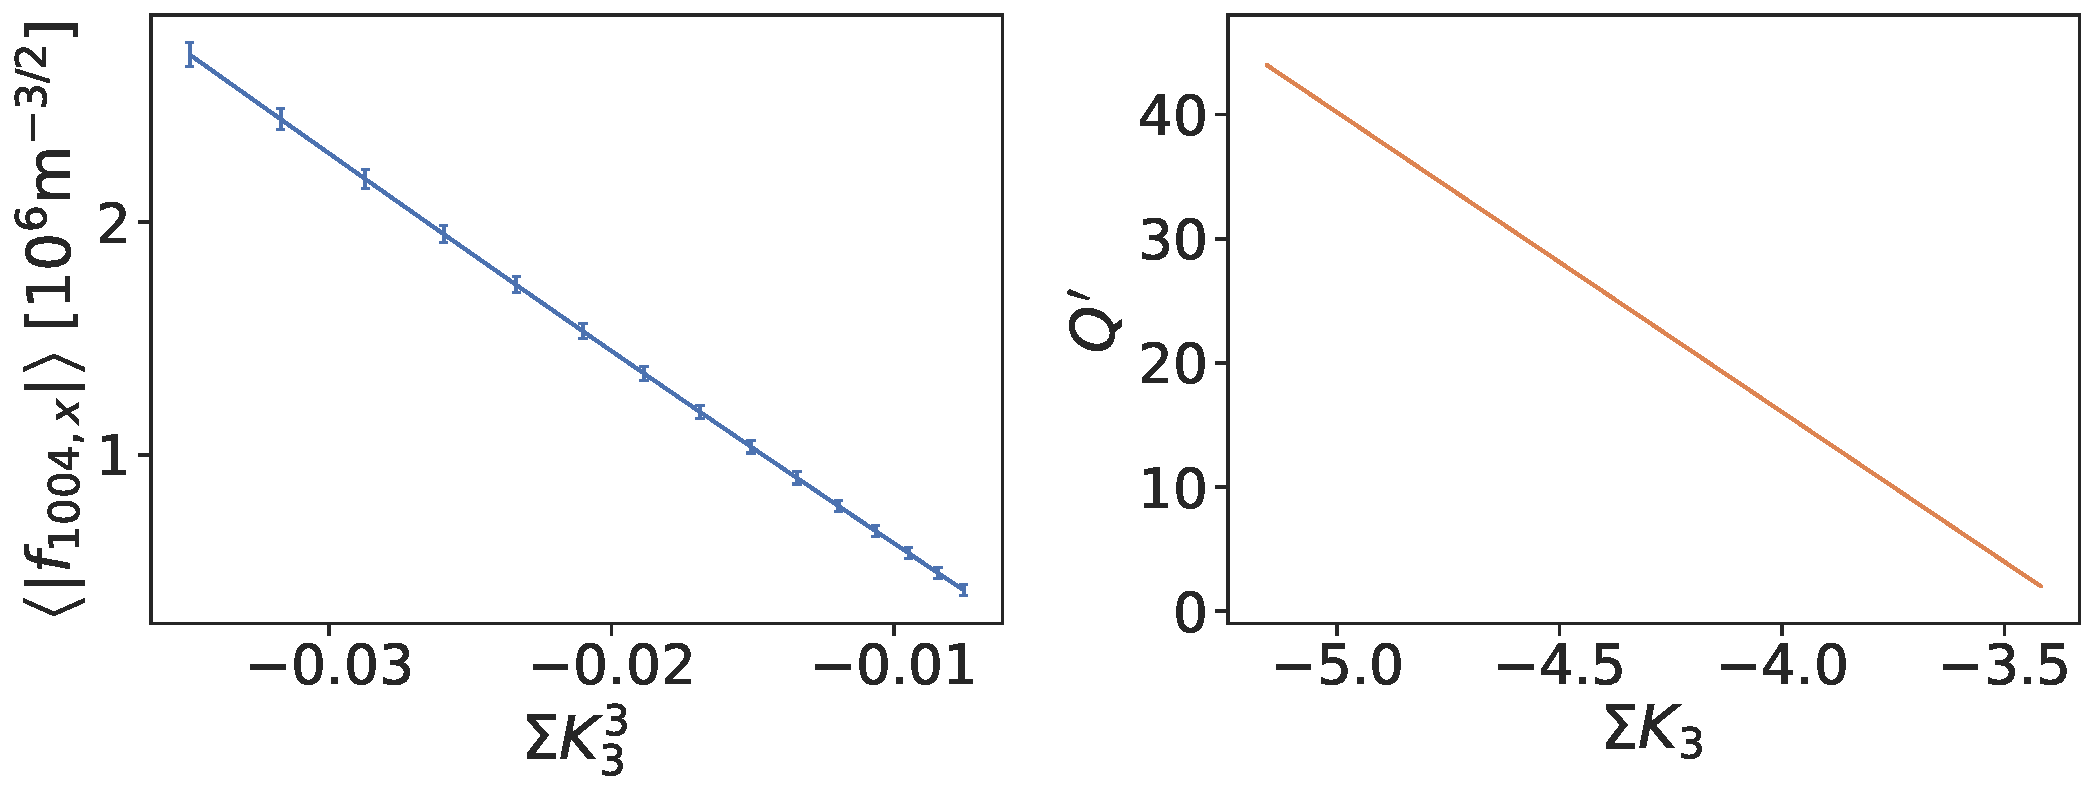
\includegraphics[width=0.9\textwidth]{./images/f1004/avg_f1004_k3.pdf}
    \caption{Average amplitude of the decapolar RDT $f_{1004}$ depending on the overall strength
    of the sextupoles used to control the linear chromaticity $Q'$. The right plot can be used
    to relate the RDT amplitude to a specific $Q'$ value.}
    \label{fig:decapoles:sextupoles_k3_f1004}
\end{figure}


To confirm what is observed in simulations, measurements were performed by varying $Q'$ and kicking
the beam with the AC-Dipole. Limited by losses, up to three measurements with distinct $Q'$ were
taken, as shows \cref{fig:decapoles:rdts:measured_f1004_from_sextupoles}.

\begin{figure}[!htb]
    \centering
    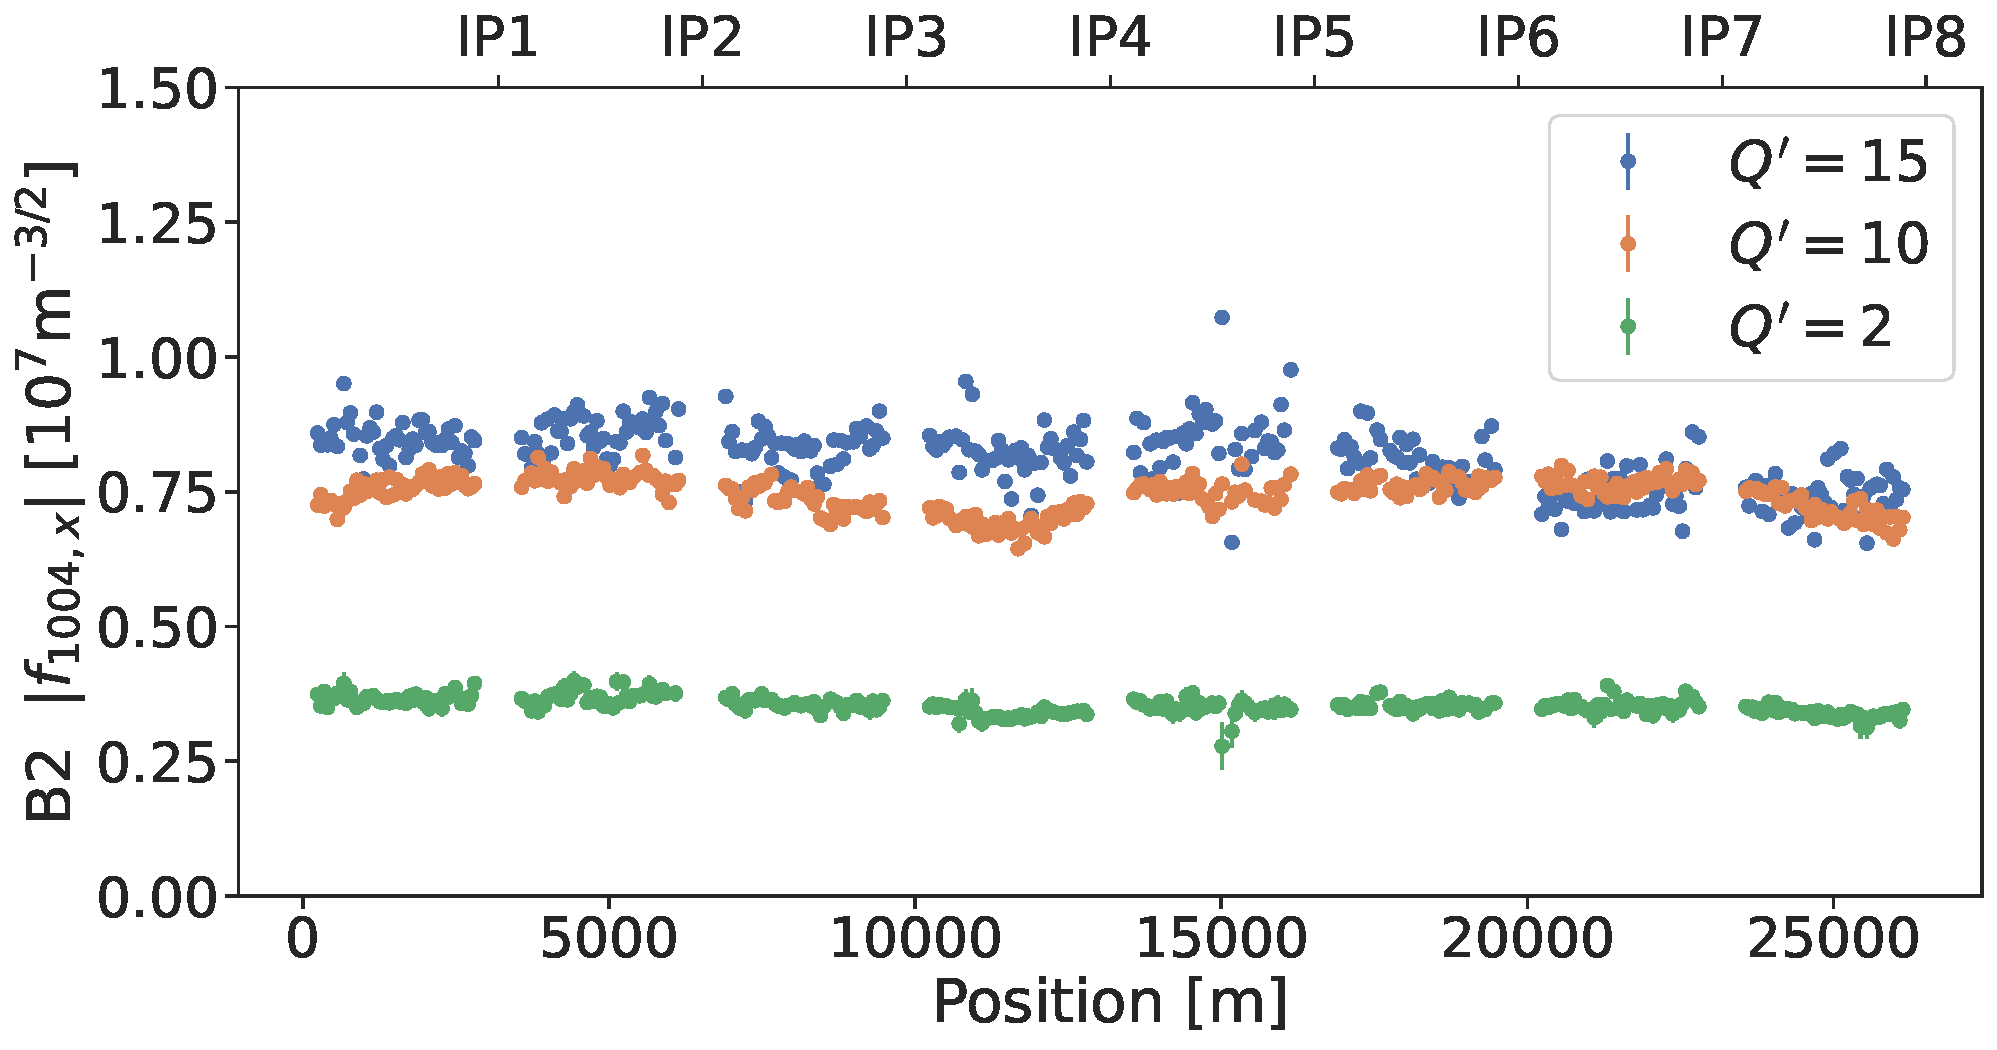
\includegraphics[width=0.85\textwidth]{./images/f1004/f1004x_q2_q10_q15.pdf}
    \caption{Measured change of the decapolar RDT $f_{1004}$ depending of the desired linear
    chromaticity $Q'$ generated by sextupoles. It is to be noted that the vertical axis is one
    order of magnitude higher than the previous simulations' plot.
    }
    \label{fig:decapoles:rdts:measured_f1004_from_sextupoles}
\end{figure}

Like in simulations, it is observed that an increase in $Q'$ translates to an increase in 
$|f_{1004}|$. The scale of the amplitude is though one order of magnitude higher than that of
simulations. An offset for all measurements could be explained by non-included field-errors. The
shift between them however should be similar between machine and simulations, this could be
due by the interaction of the sextupolar fields with octupoles, as detailed in the following
section. More data points with varying $Q'$ at similar kick amplitudes would be required to further
investigate.


% ------- Sextupole + Octupole ----------
\subsubsection{\review{Sextupoles and Octupoles}}


At the second order of the BCH expansion, the combination of a sextupole and an octupole yields a
decapolar-like expression.
Like sextupoles, octupoles are used in operation, thus contributing to decapolar fields. This
happens amongst other when correcting the second order chromaticity $Q''$ and most importantly with
the Landau Octupoles, which are powered to high strengths at injection energy to introduce Landau
damping~\cite{gareyte_landau_1997}.
Derivation of such a combination can be found in
\cref{appendix:transfer_map:sextupole_and_octupole}. The resulting Hamiltonian indeed is similar to
the terms of a decapole, dropping the $p_{x,y}$ terms for readability:

\begin{equation}
    \begin{aligned}
         H_3 H_4 &\propto \frac{1}{24} \left(x^5 + 2x^3y^2 + xy^4 \right)\\
                   &\sim    x^5 - 10x^3y^2 + 5xy^4.
    \end{aligned}
    \label{eq:decapoles:sextupole_octupole_b5}
\end{equation}

In order to assess the previous equation, simulations were run with several configurations.
As seen previously, a combination of two sextupoles creates a decapolar-like field, varying their 
field is thus not needed. Rather, a set of two configurations was run to check the impact of 
octupoles alone. The first configuration is ran with all sextupoles of the machine
turned off, while octupoles are powered. The second configuration turns off all sextupoles and
octupoles. \cref{fig:decapoles:rdts:sectupole_octupole_no_diff} shows the resulting RDT $f_{1004}$
from these simulations. It is there apparent that varying octupoles without sextupoles does not have 
any effect on this RDT.

\begin{figure}[!htb]
    \centering
    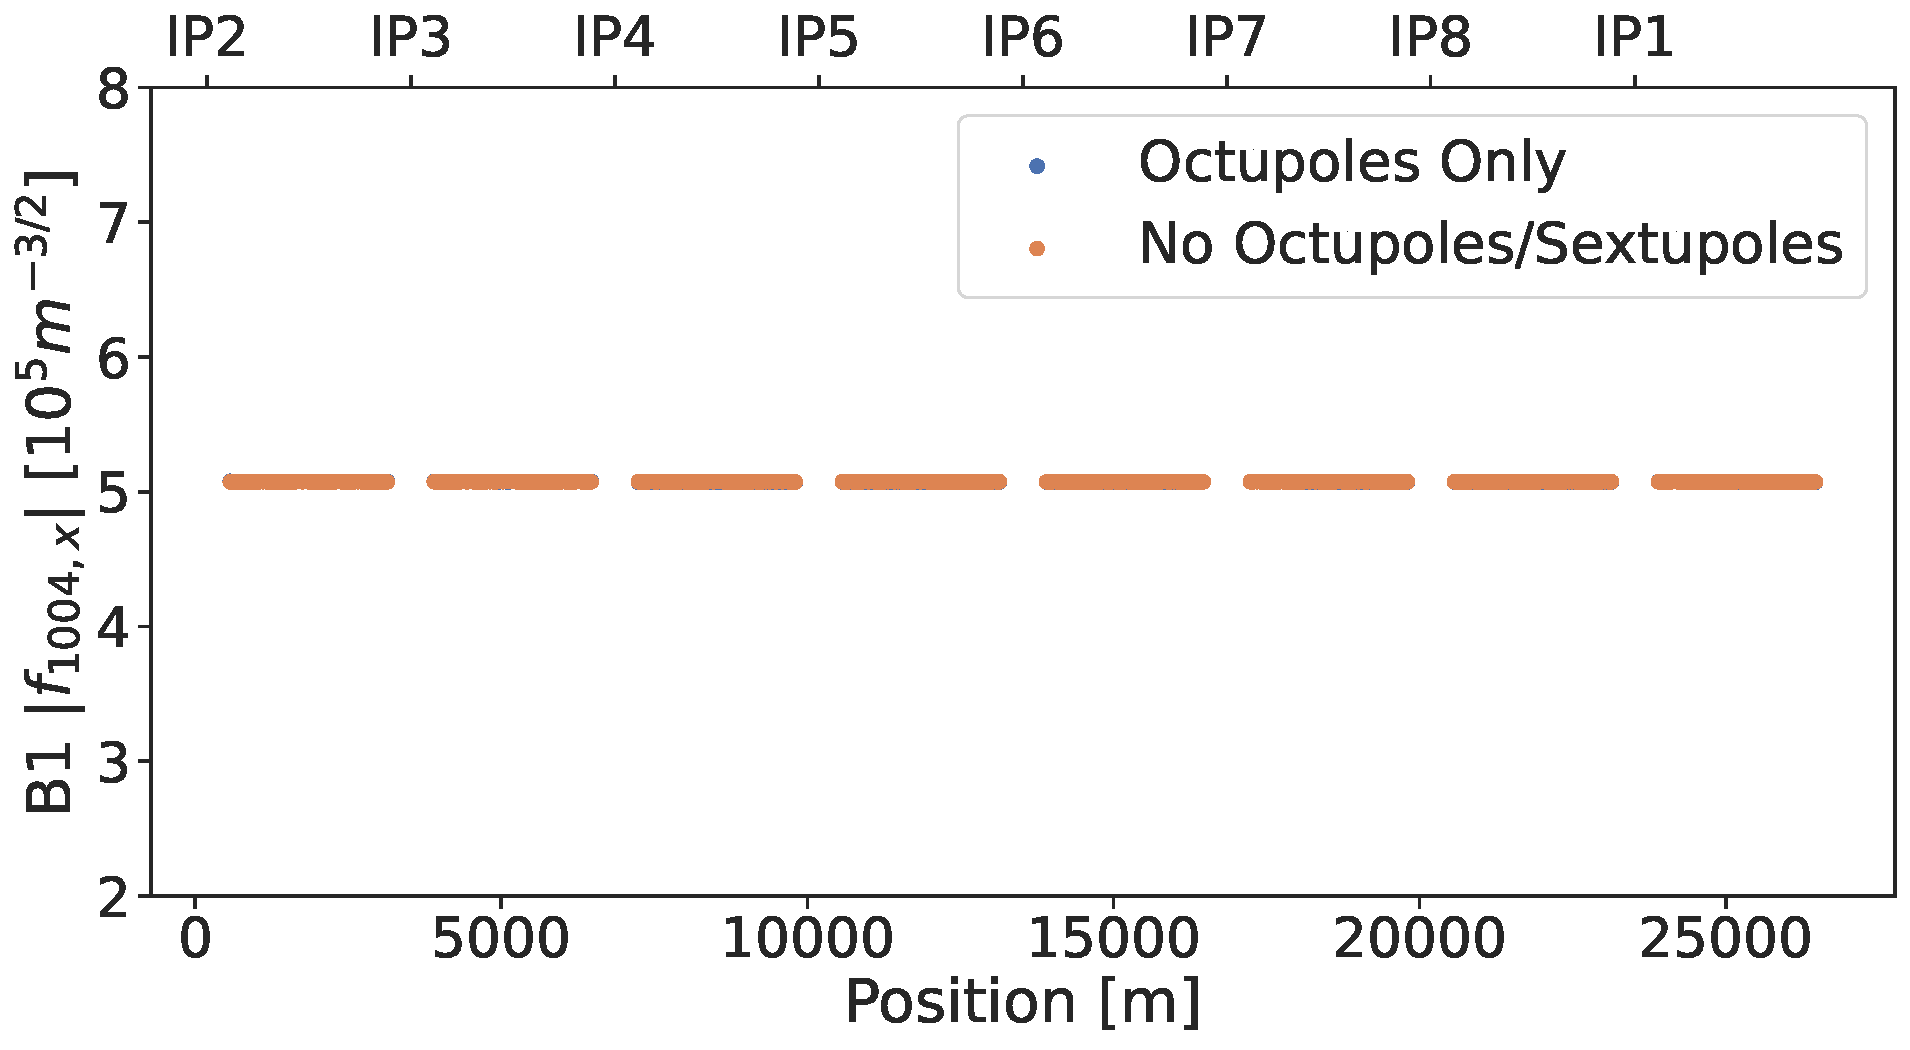
\includegraphics[width=0.8\textwidth]{./images/f1004/f1004_no_ms.pdf}
    \caption{Simulated decapolar RDT $f_{1004}$ with two different schemes. First scheme has
    lattice sextupoles turned off and octupoles turned on. Second scheme has all sextupoles of the
    lattice turned off and octupoles turned off as well. No difference is seen, as expected from
    the equations.}
    \label{fig:decapoles:rdts:sectupole_octupole_no_diff}
\end{figure}

The most powerful octupoles used in operation are the lattice octupoles, used for Landau damping.
\cref{fig:decapoles:rdts:simulation_mo_powered} shows a simulation ran with varying strengths of
those magnets. It can be noted here that the shift of the RDT is almost of an order of magnitude,
making octupoles a large contributor to the decapolar fields.

\begin{figure}[!htb]
    \centering
    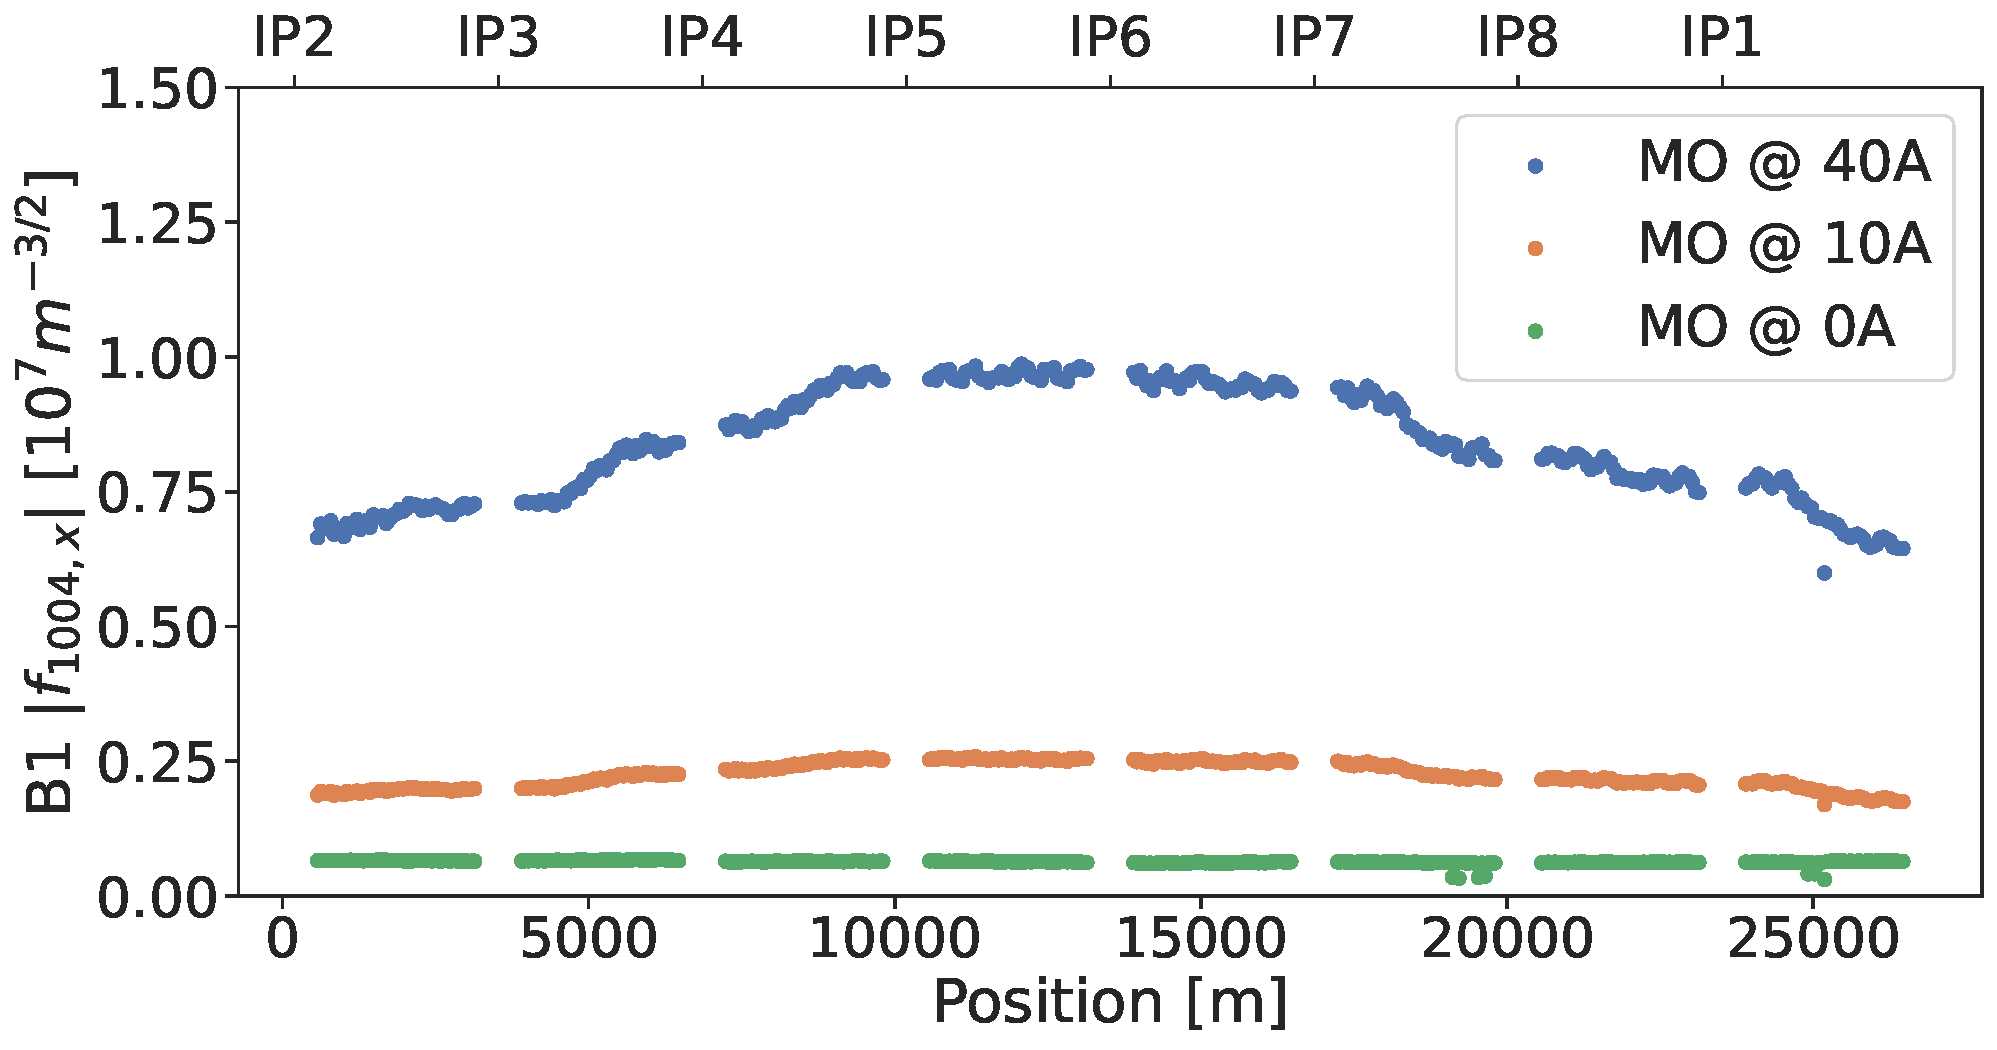
\includegraphics[width=0.8\textwidth]{./images/f1004/f1004_mo.pdf}
    \caption{Simulated change of the decapolar RDT $f_{1004}$ depending of the strength of the
    lattice octupoles used for Landau damping.}
    \label{fig:decapoles:rdts:simulation_mo_powered}
\end{figure}

While decapoles are expected to be the main contributors to decapolar fields, other strong sources
can indeed be identified. \cref{fig:decapoles:rdts:contributions} shows the average amplitude of the
RDT $f_{1004}$ depending on the error sources introduced in the simulations. A large contribution
comes from the octupolar errors in the main dipoles, being actually larger than the decapolar errors
in those magnets.

\begin{figure}[!htb]
    \centering
    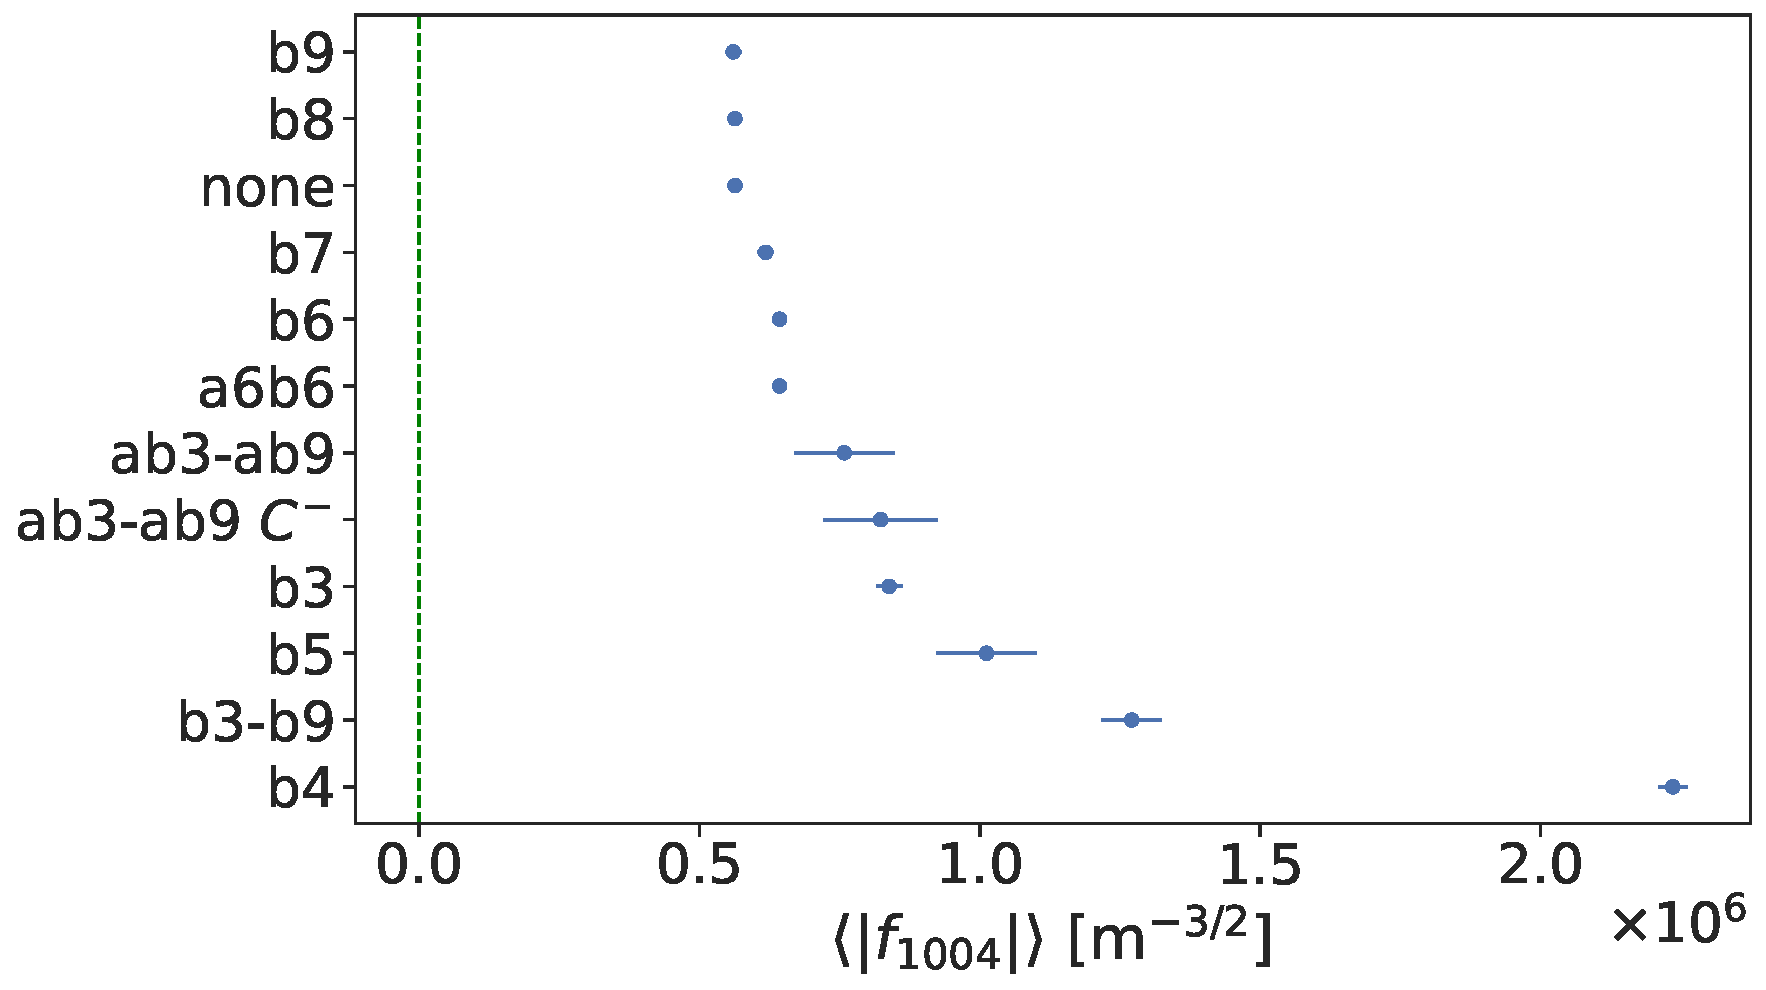
\includegraphics[width=0.8\textwidth]{./images/f1004/f1004_several_factors.pdf}
    \caption{Simulation of the amplitude of the decapolar RDT $f_{1004}$ depending on the field
             errors applied on main dipoles as well as coupling ($C^-$). While it is apparent that
             some multipolar errors drive the resonance higher, some combinations actually seem to
             cancel each other.}
    \label{fig:decapoles:rdts:contributions}
\end{figure}

\begin{wraptable}{r}{0.4\textwidth}
    \centering
    \begin{tabular}{rr}
    \toprule
    Factor & RMS $|f_{1004}|$ \\
    \midrule
       -10 & $37,308,159$         \\ 
        -4 &  $6,721,270$          \\ 
         0 &  $3,533,796$          \\ 
        -1 &  $2,333,384$          \\
    \bottomrule
    \end{tabular}
    \caption{RMS of $|f_{1004}|$ depending on the factor of the $Q''$ corrections.}
    \label{table:decapoles:corrections_dq2_f1004_rms}
\end{wraptable}

Measurements were performed to confirm and quantify the effect of octupoles coupled with sextupoles
on the decapolar fields. Previous corrections, aimed at correcting the second order chromaticity
$Q''$, via octupolar correctors \textit{MCO}, were applied with varying factors. Such corrections
apply use a uniform trim on all correctors of $\approx +2.5K_4$.
\cref{decapoles:rdts:measured_f1004_mco} shows a comparison of the resulting RDT with those
corrections at factors $-10$, $-4$, $-1$ and $0$.

\begin{figure}[!htb]
    \centering
    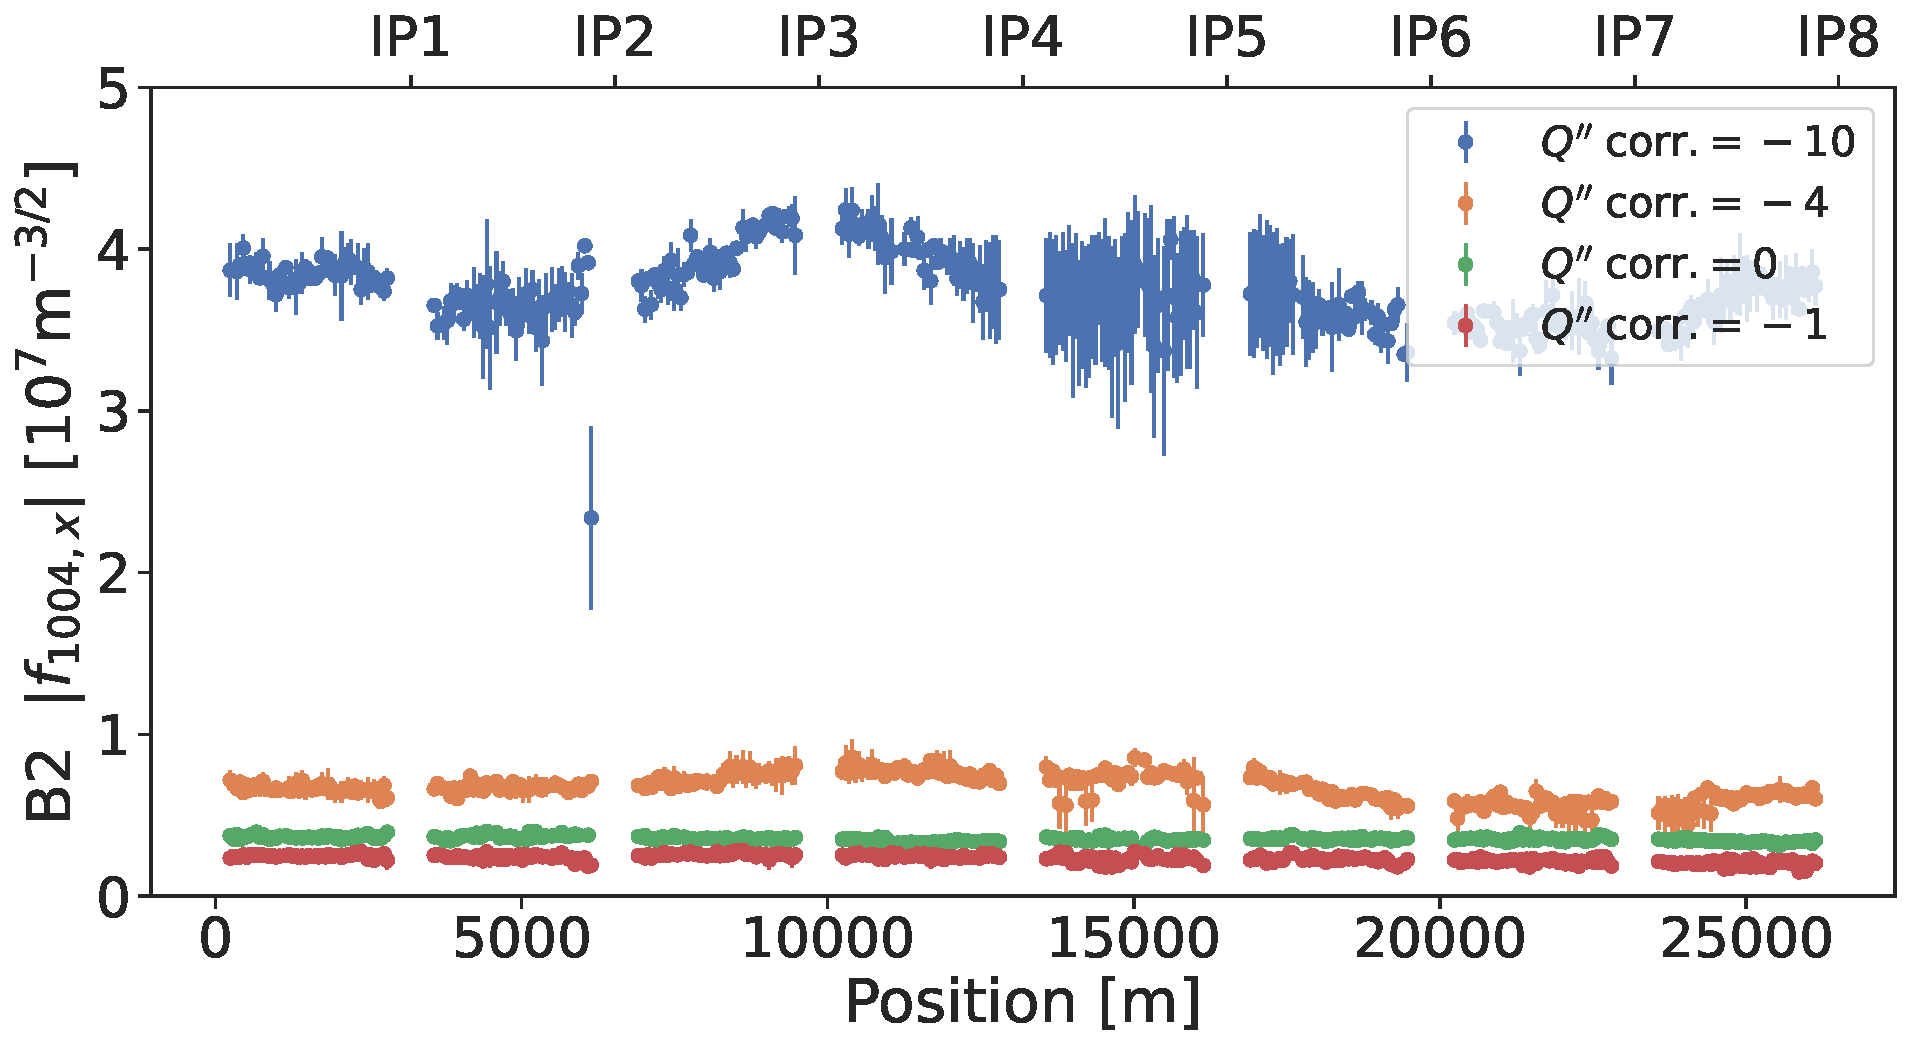
\includegraphics[width=0.8\textwidth]{./images/f1004/f1004x_mco_corr.pdf}
    \caption{Shift of the decapolar RDT $f_{1004}$ depending on the factor applied on octupolar
    corrections for $Q''$.}
    \label{decapoles:rdts:measured_f1004_mco}
\end{figure}


  
\cref{table:decapoles:corrections_dq2_f1004_rms} shows the RMS of the amplitude of this RDT for the 
various configurations. Similar to the shift observed when powering the landau octupoles in
simulations, the shift is of one order of magnitude between factors $-0$ and $-10$. Measurements
with landau octupoles were also attempted but losses made it impossible to obtain high enough
amplitudes to correctly measure the RDT.

Simulated and observed large shifts due tu octupoles are relevant to the operation of the LHC, as
resonances can be greatly deteriorated, especially when powering landau octupoles.
A better understanding of the interaction between Landau octupoles and octupolar correctors could
lead to improved corrections in not only octupolar but also decapolar fields in the future.


%==================================
%             Impact
%==================================
% === Impact / Lifetime
\section{\todo{Impact of Decapolar Fields}}

Decapolar fields can influence the beam lifetime in several ways. Chromatic amplitude detuning and
chromaticity will induce a tune shift, relative to either or both the action and the momentum
offset. After such detuning, particles may move closer to certain resonances in tune space, causing
their oscillations to grow, eventually leading to their loss.


% ============================================
%                 Large RDT
% ============================================
\subsection{\review{Large RDT}}

\begin{wraptable}{r}{0.4\textwidth}
    \centering
    \begin{tabular}{rr}
    \toprule
    $\Delta K_5$         & RMS $|f_{1004}|$ \\
    \midrule
    $0$                  &            $618,947$ \\
    $\pm10500$             &         $17,566,377$ \\
    $\mp10500$             &         $17,623,867$ \\
    \bottomrule
    \end{tabular}
    \caption{RMS of $|f_{1004}|$ relative to the powering scheme of decapolar correctors.}
    \label{table:decapoles:impact:rdt_amplitude}
\end{wraptable}

As seen previously in \cref{fig:decapoles:rdts:tune_diagram}, the resonance $1Q_x - 4Q_y$ passes
through the beam in tune space, deteriorating the lifetime of the nearby particles.
In order to measure the impact of this resonance on the beam, a knob was created, alternating the 
current of all decapole correctors in the machine arc by arc. Such a powering scheme has no impact
on chromaticity as the sum of the strengths $K_5$ is zero. Rather, the RDT $f_{1004}$ is impacted.
Is it to be noted that this is not a correction, but purely a way to artificially increase the RDT
in order to quantify the effect of the resonance.

Starting with nominals corrections for $Q'''$ corrections, a delta of $\pm 10500 K_5$ is applied on
each decapolar correctors. \cref{fig:decapoles:impact:alternating_knob} shows the response of the
real part of the RDT for this scheme and its inverse. The amplitude of the RDT is on a similar level
as the shift is significantly larger than the original level of the RDT.
\cref{table:decapoles:impact:rdt_amplitude} indicates the amplitude of the RDT created with each
knob value.

\begin{figure}[!htb]
    \centering
    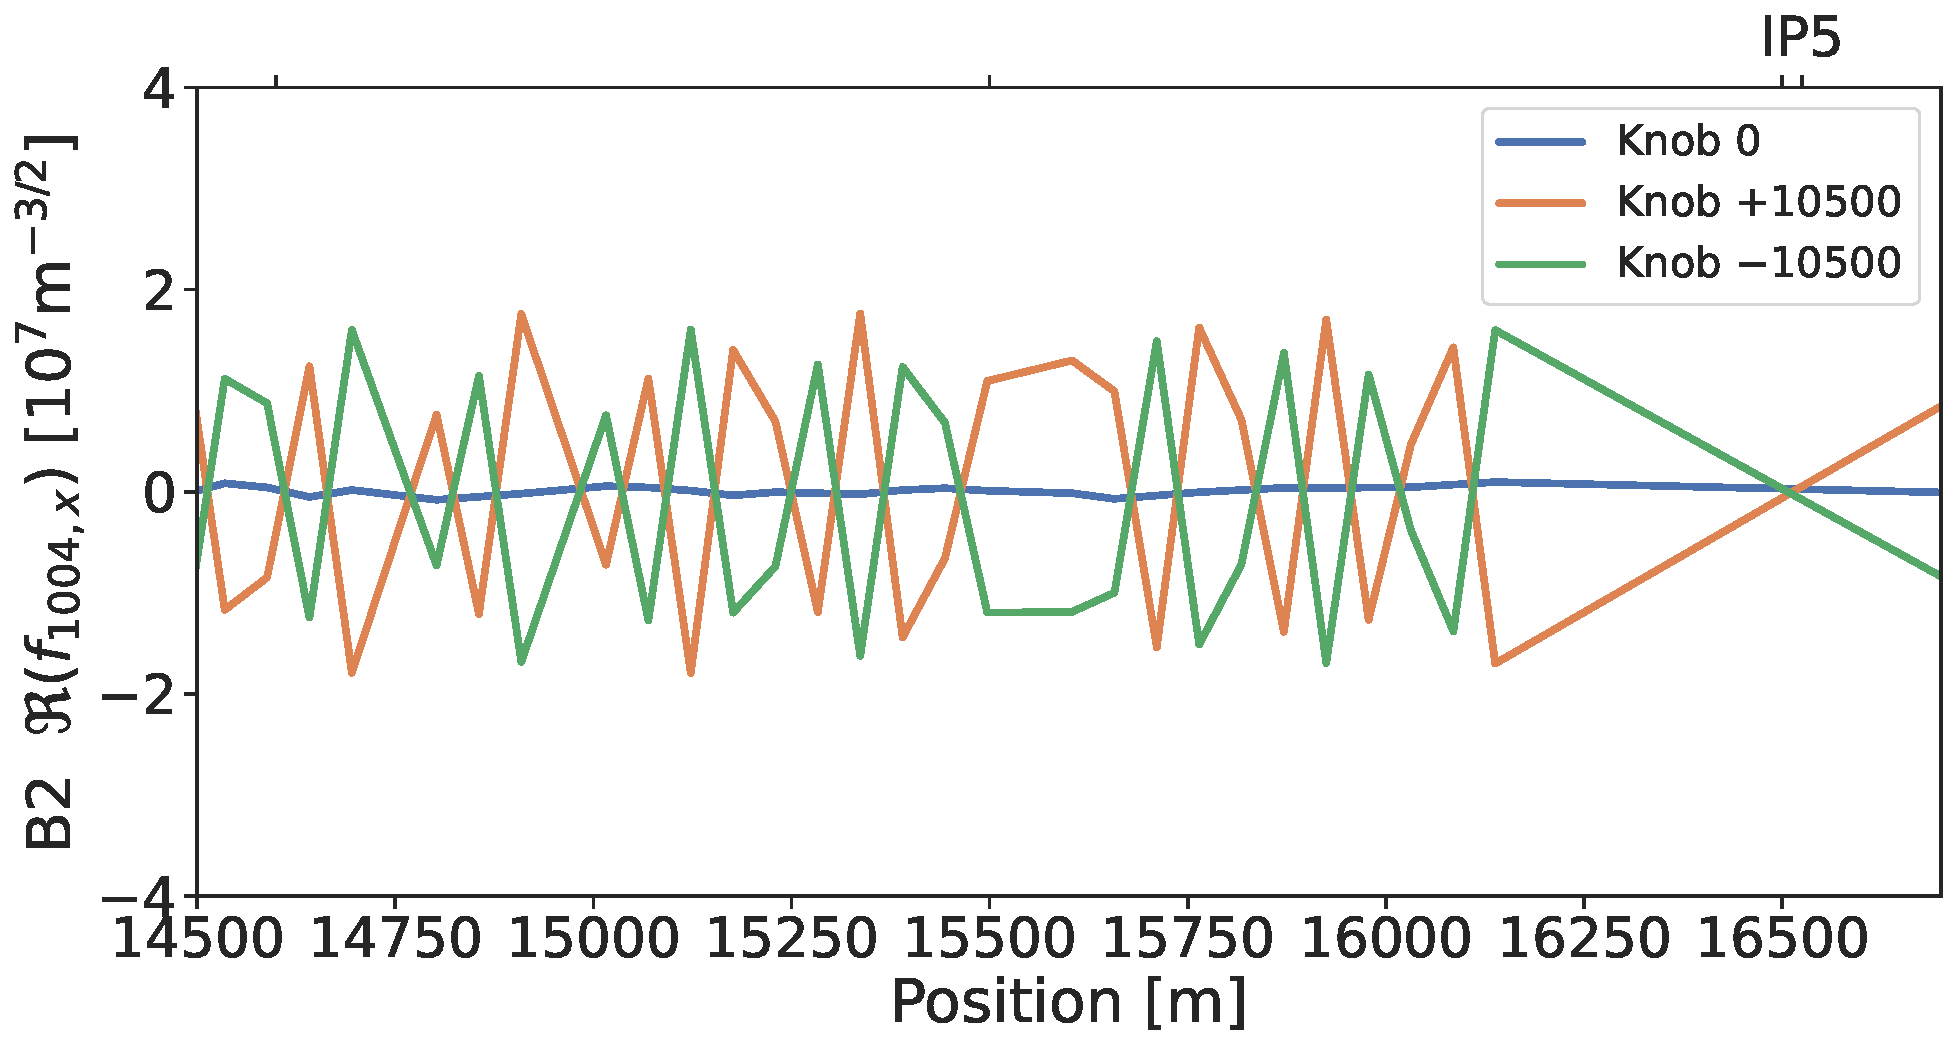
\includegraphics[width=0.8\textwidth]{./images/f1004/f1004x_knob_alt_lifetime_real.pdf}
    \caption{Measured real part of the RDT $f_{1004}$ depending on the powering scheme of the decapolar
    correctors.}
    \label{fig:decapoles:impact:alternating_knob}
\end{figure}

In order to measure the lifetime, a long period must be allocated as the signal returned from
monitors can be jittery. \cref{fig:decapoles:impact:b5_lifetime} shows this lifetime depending on
the decapolar strength scheme applied. The current of only one circuit is shown for readability.
A current of $\approx 230$ corresponds to a knob value of $+10500$ while a current of $-45$
corresponds to $0$.

\begin{figure}[!htb]
    \centering
    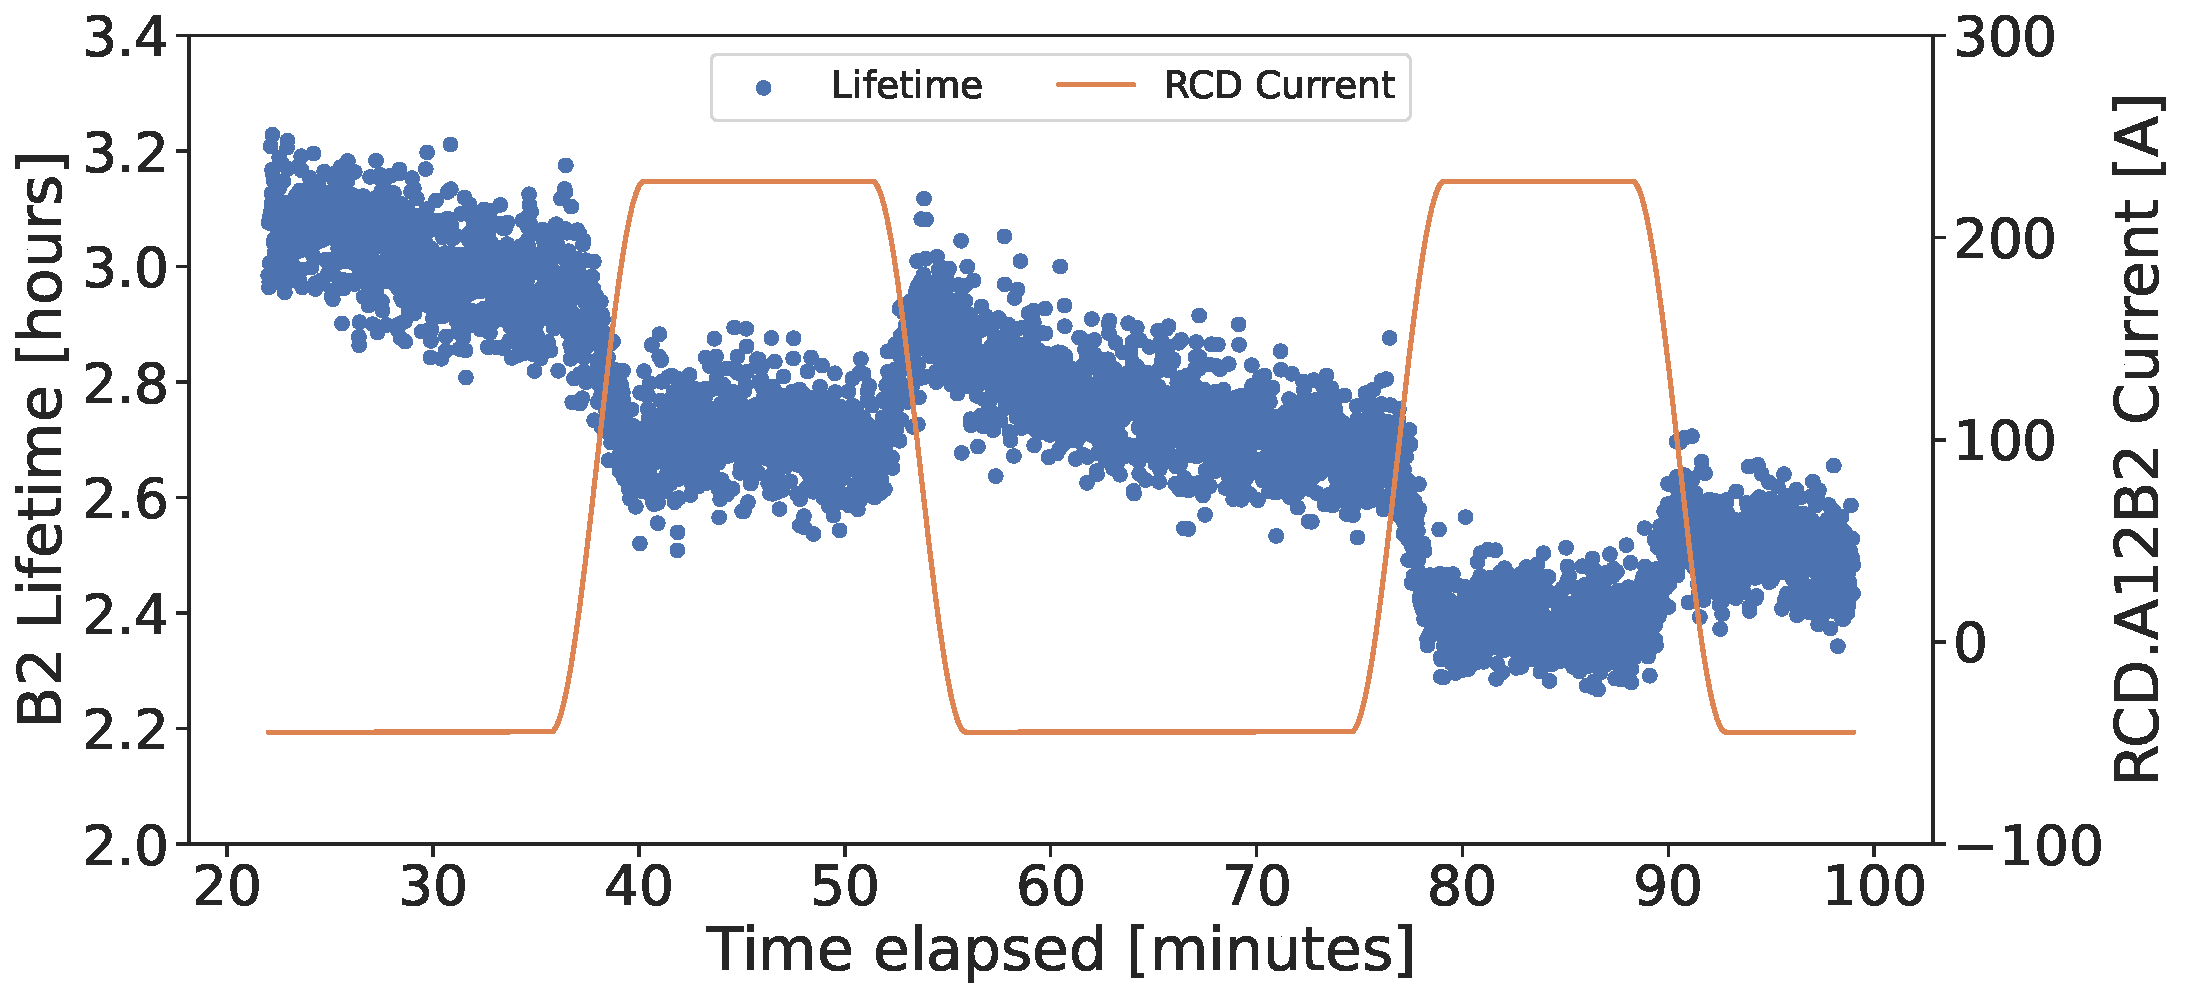
\includegraphics[width=0.8\textwidth]{./images/b5_lifetime.pdf}
    \caption{Measured lifetime of Beam 2 upon application of two different powering schemes for
    decapolar correctors. One trim keeps the RDT at a low amplitude while the other greatly
    amplifies it.}
    \label{fig:decapoles:impact:b5_lifetime}
\end{figure}

It is clear from this measurement that a large RDT decreases the lifetime of the beam.
The first pair of trim sees the average lifetime decreasing of $0.31 \pm 0.03$ hours, while the
second one sees a decrease of $0.36 \pm 0.03$ hours. This observed decrease of 20 minutes accounts
for $10\%$ of the beam lifetime at injection energy.



% ============================================
%                Corrections
% ============================================
\subsection{\todo{Corrections}}

In order to understand what can be gained from correcting decapolar fields, a lifetime measurement
was taken with the corrections described in 
\cref{section:decapoles:decapolar_contribution_correction}. This scheme corrects the three decapolar 
observables, being the RDT $f_{1004}$ linked to the resonance $1Q_x - 4Q_y$, the third order
chromaticity $Q'''$ and the chromatic amplitude detuning terms.

\cref{fig:decapoles:impact:b5_lifetime_rdt_corr} shows the evolution of the lifetime, starting with
corrections applied, removed and then trimmed to their opposite. A net change in lifetime for Beam 1
can be measured after each application. Acquired signal for Beam 2 has been deemed to noisy to be 
relevant, due to the shortness of the measurement.

\begin{figure}[!htb]
    \centering
    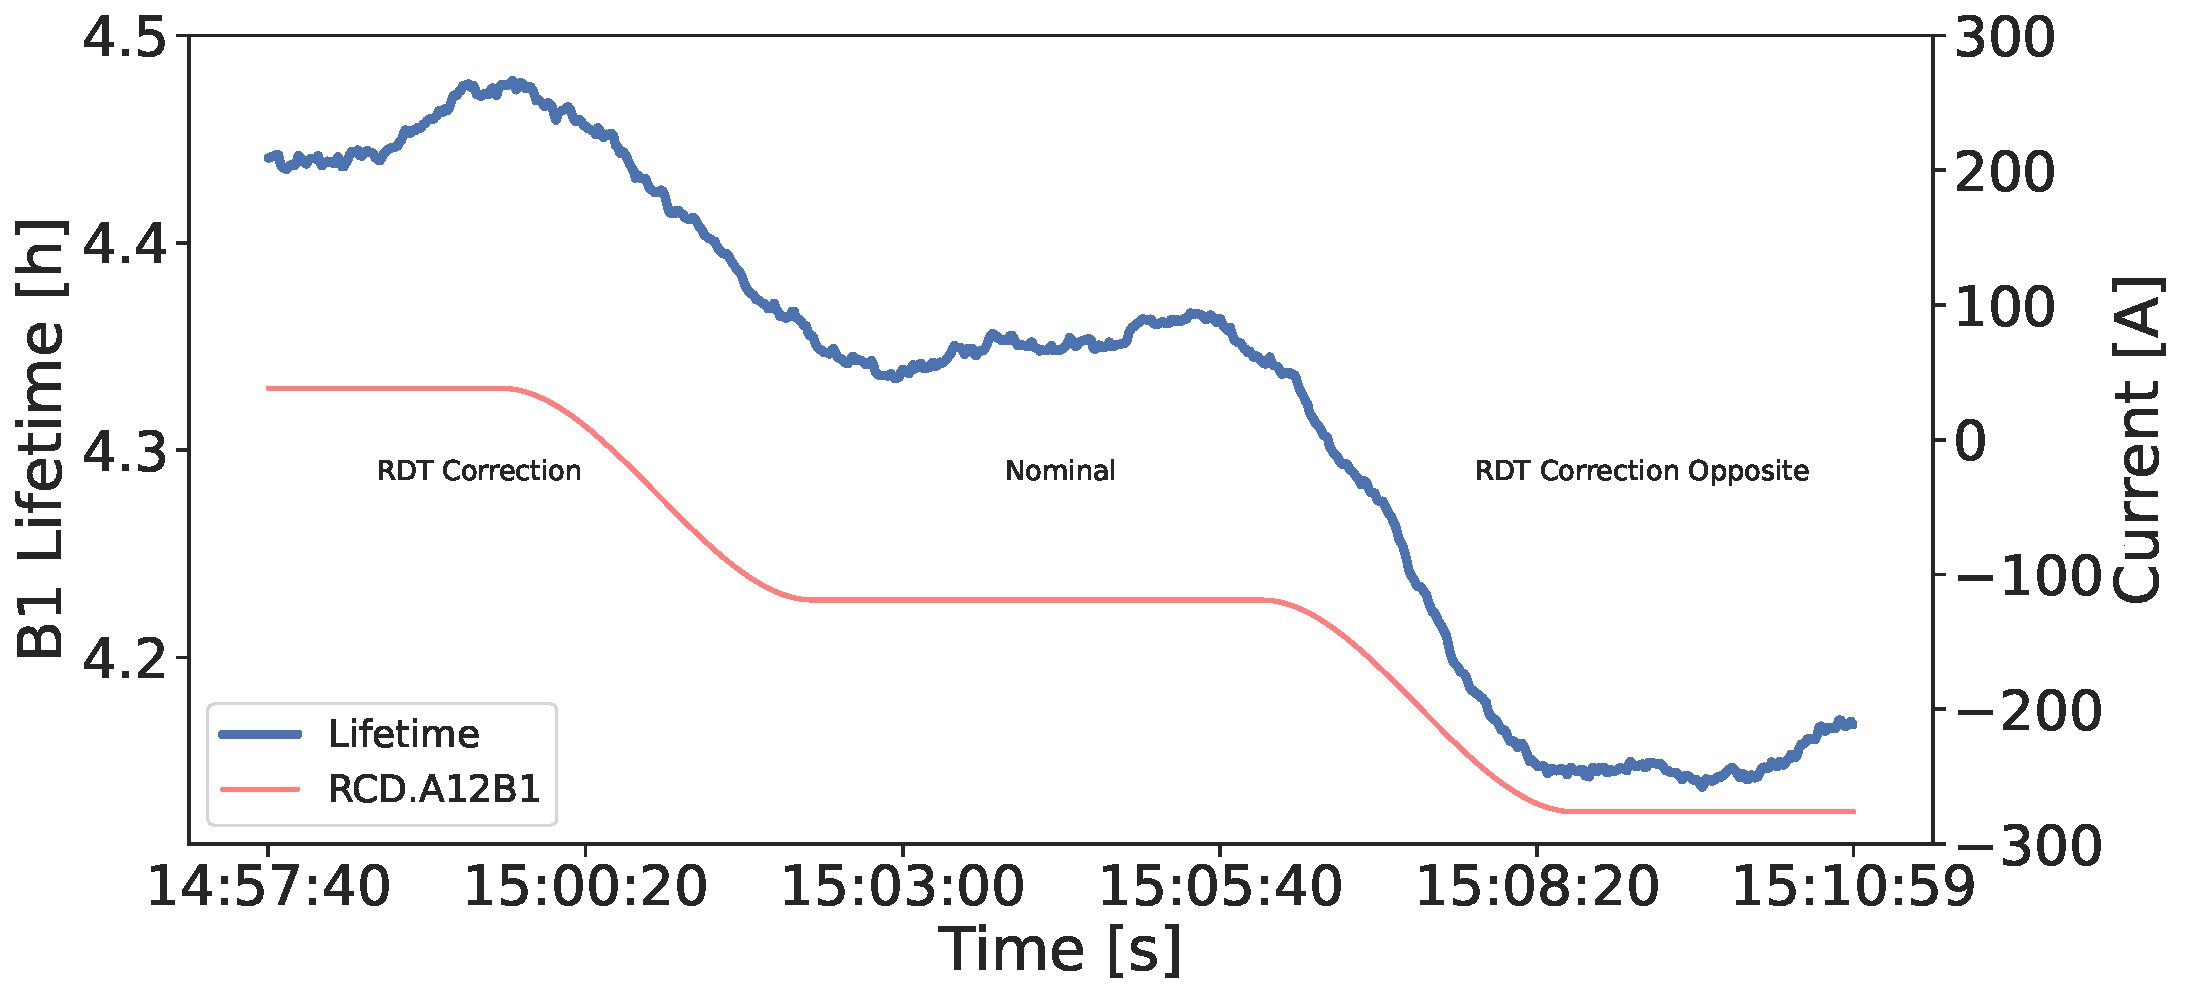
\includegraphics[width=0.8\textwidth]{./images/b5_lifetime_rdt_corr.pdf}
    \caption{Measured lifetime of Beam 1 with the nominal corrections for $Q'''$, combined
    correction of $f_{1004}$ and $Q'''$, and its inverse.}
    \label{fig:decapoles:impact:b5_lifetime_rdt_corr}
\end{figure}

It is apparent here that the corrections have a beneficial effect on the Beam. The lifetime
improvement is of $\approx 3 \%$, while the degradation after applying the opposite is of $\approx
5\%$.

% 2023-06-14

% ---------------------------------------
%             subsection
% ---------------------------------------



